\documentclass[conference,a4paper]{IEEEtran}
\IEEEoverridecommandlockouts
\usepackage{fontspec}
\setmainfont{Times New Roman}
\setmonofont{Courier New}[Scale=0.85]
\usepackage{amsmath,amssymb}
\usepackage{graphicx}
\usepackage{array,tabularx}
\usepackage[hyphens]{url}
\usepackage{cite}
\usepackage{xcolor}
\usepackage{balance}
\renewcommand{\tabularxcolumn}[1]{p{#1}}
\setlength{\tabcolsep}{3pt}
\urlstyle{tt}
\sloppy

\begin{document}

\title{Fairness Audit of Entity-Level Resume Matching}
\author{\IEEEauthorblockN{Ajinkya Phatak}
\IEEEauthorblockA{Registration No. 23BCE0643}}

\maketitle

\begin{abstract}
Semantic resume–job matchers usually embed the whole resume, so a candidate's name, pronouns and style of self-description can move the match score. We test whether restricting the comparison to extracted skill entities reduces that leakage. Our matcher extracts skill and knowledge entities from both texts (a JobBERT tagger fine-tuned on SkillSpan, the ESCO taxonomy and filtered noun chunks), embeds each entity with JobBERT-v2, and scores a pair by IDF-weighted MaxSim late interaction.

We audit it against seven other matchers with a counterfactual design. Each of 16,217 BiasBios biographies in 234 held-out job pools is rewritten seven ways (pronoun swap, three name swaps, affiliation swap, agentic-to-communal wording, full gender flip), and we measure how far each matcher's score moves, in units of the pool's score standard deviation.

Under the full gender flip the entity-level matcher moves by 0.033 pool SDs, against 0.121–0.181 for four full-text neural matchers and 0.272 for the deployed application's original matcher (Holm-corrected p < 0.001 for each). Its ranking accuracy is competitive but not the best: nDCG@10 is 0.619, above MiniLM (0.602) and BM25 (0.541) and below full-text JobBERT-v2 (0.716). Lexical matchers move even less (0.001–0.005), because pronouns are stop-words for them, but rank worse.

The hypothesis therefore holds against neural full-text matching and fails against lexical matching. Ablations show that the choice of extractor decides what leaks. The method now runs in the accompanying web application, which lets a user repeat the audit on their own resume.

\end{abstract}
\begin{IEEEkeywords}resume matching, algorithmic hiring, counterfactual fairness, late interaction, skill extraction, BiasBios\end{IEEEkeywords}
\section{Introduction}
\subsection{Motivation}
Automated screening tools rank candidates by how well a resume matches a job description. Keyword tools miss paraphrases, so current systems use sentence embeddings: the whole resume and the whole posting each become one vector, and the cosine between them is the score.

That design has a side effect. Everything in the resume enters the vector: the skills, but also the candidate's first name, their pronouns, the clubs they joined and how assertively they write. None of these is a qualification. If any of them shifts the vector, it shifts the score, and two candidates with identical skills are ranked differently.

This is the algorithmic form of a well-documented human bias. Field experiments that send identical resumes under different names find different callback rates \cite{bertrand}, and recent audits find the same pattern in embedding-based resume retrieval \cite{wilson}.

\subsection{Baseline System}
The project began as a working web application, a FastAPI backend with a Next.js frontend, that scored a resume against a job description. Its matcher already had the right instinct: it extracted phrases from both texts and compared phrase to phrase rather than document to document. But it extracted every noun chunk, so pronouns such as ``She'', employer names and cities became ``skills'', and its thresholds (0.55 for a match, 0.35–0.55 for a near-miss) were hardcoded and untested.

That raised a research question worth answering properly: if a matcher only ever sees extracted skills, does it leak less demographic signal than one that sees the full text, and what does that cost in accuracy?

\subsection{Approach Overview}
We turned the application into a reproducible research codebase and ran a counterfactual fairness audit in eight phases:

\begin{enumerate}
\item Audited the existing matcher and documented its behaviour and bugs.
\item Built and evaluated four skill extractors, including a fine-tuned token classifier.
\item Assembled an evaluation set from BiasBios biographies and LinkedIn job postings.
\item Implemented eight matchers behind one interface.
\item Generated seven counterfactual rewrites of every candidate.
\item Measured ranking accuracy and score shifts with confidence intervals and paired tests.
\item Ran ablations, selected the final method on development data only, and checked it on untouched test pools.
\item Rebuilt the web application on the final method, with a research page and a per-resume fairness check.
\end{enumerate}
\subsection{Contributions}
\begin{itemize}
\item A counterfactual audit of eight resume–job matchers on 234 test pools, with seven perturbation conditions, cluster-bootstrap confidence intervals and Holm-corrected paired tests.
\item Evidence that entity-level late interaction leaks less gender and name signal than every full-text neural matcher tested, at competitive accuracy, and that it does not beat lexical matchers on leakage.
\item An ablation showing that the extractor, not the encoder or the aggregation, decides which demographic cues reach the score.
\item A data-driven replacement for a hardcoded ``near-miss'' suggestion band, validated against the ESCO hierarchy.
\item An open, tested codebase and a deployed application that runs the audited method and exposes the audit to end users.
\end{itemize}
The matching mechanism itself, MaxSim late interaction, is not ours. It comes from ColBERT \cite{colbert} and BERTScore \cite{bertscore}. Our contribution is applying it to extracted skill entities and auditing the result.

\section{Related Work}
Five lines of work meet in this project. For each, we say what it established and how we use it.

\subsection{Resume–Job Matching}
Early matching was lexical. BM25 \cite{bm25} and TF-IDF score a document by weighted term overlap; they are fast, interpretable and blind to paraphrase. Neural person–job fit models \cite{pjfnn,apjfnn} learn representations from historical hiring decisions, which makes them accurate on their own data and prone to reproducing the biases in it.

Pretrained sentence encoders removed the need for hiring labels. Sentence-BERT \cite{sbert} and its distilled successors MiniLM \cite{minilm} and MPNet \cite{mpnet} give a single vector per text, and cosine similarity gives a score. Cross-encoders \cite{monobert} read both texts together and are usually more accurate and much slower. Domain encoders such as JobBERT \cite{jobbert} and its successor JobBERT-v2 are trained on job titles and skill lists. We use all of these as baselines.

\subsection{Late-Interaction Retrieval}
A single vector per document loses detail. ColBERT \cite{colbert} keeps one vector per token and scores a query against a document by MaxSim: for every query token take its best-matching document token, then sum. BERTScore \cite{bertscore} uses the same greedy matching to evaluate generated text, with optional IDF weighting.

Our scorer is this mechanism with one change: the units are extracted skill entities instead of all tokens. We cite both papers and do not claim the mechanism.

\subsection{Skill Extraction}
Skill extraction turns free text into the units we match. Two resources matter here. ESCO, the European Commission's taxonomy, lists about 13,900 skill and knowledge concepts with alternative labels and a broader/narrower hierarchy. SkillSpan \cite{skillspan} provides job postings annotated with skill and knowledge spans, and shows that domain-adapted BERT models, including their own JobBERT (BERT further pretrained on job postings), outperform general ones on span extraction. We evaluate on SkillSpan and fine-tune that model.

\subsection{Bias in Hiring and Language Models}
\subsubsection{Human hiring} Resumes with white-sounding names received about 50\% more callbacks than identical resumes with African-American-sounding names \cite{bertrand}. Gaucher, Friesen and Kay \cite{gaucher} showed that job advertisements use gendered wording and that masculine-coded wording lowers women's interest in a job. Madera, Hebl and Martin \cite{madera} found that recommendation letters describe women in communal terms and men in agentic terms, and that communal descriptions hurt hiring outcomes.

\subsubsection{Algorithmic hiring} Amazon abandoned a resume-screening model that had learned to penalise the word ``women's'' \cite{dastin}. Raghavan et al. \cite{raghavan} surveyed commercial screening vendors and found little public evidence of validation. Wilson and Caliskan \cite{wilson} audited embedding-based resume retrieval and found strong preferences by name-signalled race and gender.

\subsubsection{Representations} Word embeddings encode gender stereotypes \cite{bolukbasi}. De-Arteaga et al. \cite{biasbios} released BiasBios, about 400,000 online biographies labelled with occupation and gender, and showed that occupation classifiers have gender gaps in true-positive rate that persist after removing explicit gender words. BiasBios is our candidate corpus, and the TPR gap is one of our metrics.

\subsection{Counterfactual Evaluation}
Counterfactual fairness \cite{kusner} asks that a decision stay the same in a world where the individual's protected attribute differs. For text, the practical test is perturbation: swap the attribute's surface cues and compare outputs. Counterfactual data augmentation \cite{lu,zhao} introduced bidirectional pronoun swapping; Garg et al. \cite{garg} formalised the counterfactual token fairness gap for classifiers. This mirrors the correspondence-study design used in the human experiments above.

Group metrics complement it. Equality of opportunity \cite{hardt} compares true-positive rates across groups, and fairness of exposure \cite{singh} compares the attention a ranking gives each group.

\subsection{Research Gap}
Prior audits show that full-text embedding matchers leak demographic signal. Prior systems use skill extraction to improve matching quality. To our knowledge, no study has measured whether restricting a late-interaction matcher to extracted skills reduces counterfactual leakage, with the accuracy cost reported beside it and lexical baselines included. That is the comparison this project makes.

\section{Proposed Approach}
\subsection{Hypothesis}
\begin{quote}\itshape Entity-level resume–job matching, which extracts skills first and then does late-interaction matching over entity embeddings, leaks less demographic signal into match scores than full-text embedding matchers, at competitive ranking accuracy.\end{quote}
The reasoning is simple. A full-text encoder must represent every word it reads. An entity-level matcher only represents the spans an extractor hands it. If the extractor returns ``Python'' and ``patient assessment'' but not ``she'' or ``Emily'', then swapping the pronoun or the name cannot change the inputs to the score, so it cannot change the score.

\subsection{Evaluation Design Principles}
Three decisions shaped the design.

\subsubsection{Test the claim causally, per candidate} Group statistics (do women score lower on average?) confound the matcher with the data. A counterfactual test does not: take one candidate, change only the demographic cue, and see whether the score moves. Any movement is attributable to the cue.

\subsubsection{Report accuracy on the same axis as fairness} A matcher that returns a constant is perfectly fair and useless. Every fairness number is therefore reported beside a ranking number from the same pools, and the headline figure plots one against the other.

\subsubsection{Give the hypothesis a fair chance to fail} We included lexical baselines, the application's own original matcher, and a strong domain encoder. We fixed the selection rule for the final method before running it and excluded fairness metrics from selection, since they are the outcome under test.

\subsection{Research Questions}
\begin{table}[!t]
\caption{Research Questions}
\label{tab:1}
\centering
\footnotesize
\begin{tabularx}{\columnwidth}{l>{\raggedright\arraybackslash}Xl}
\hline
\textbf{} & \textbf{Question} & \textbf{Answered in} \\
\hline
RQ1 & Does entity-level matching shift less than full-text matchers under gender and name counterfactuals? & Section V-A \\
RQ2 & What does it cost in ranking accuracy? & Section V-A \\
RQ3 & Which component (extractor, entity types, encoder, aggregation) controls the leakage? & Section V-B \\
RQ4 & Is the application's near-miss suggestion band (0.35–0.55) justified, and what should replace it? & Section V-D \\
\hline
\end{tabularx}
\end{table}
\subsection{Falsification Criteria}
\begin{itemize}
\item The entity matcher's counterfactual gap is not significantly below the neural full-text matchers' gaps.
\item Its ranking accuracy falls to the level of the weakest baselines.
\item Its apparent fairness comes from finding no entities at all (a score of 0 before and after any rewrite). We found exactly this risk during development, and Section IV-E describes how we handled it.
\end{itemize}
\subsection{Scope of Contribution}
We do not claim late interaction, MaxSim, IDF weighting or skill extraction. The contribution is the entity-restriction hypothesis, the audit that tests it, and the finding about which component matters.

\section{System Design and Methodology}
The work ran in eight phases, each ending with a report and a decision before the next began. Sections IV and V follow that order. The final method is shown first so the rest can be read against it.

\begin{figure*}[!t]
\centering
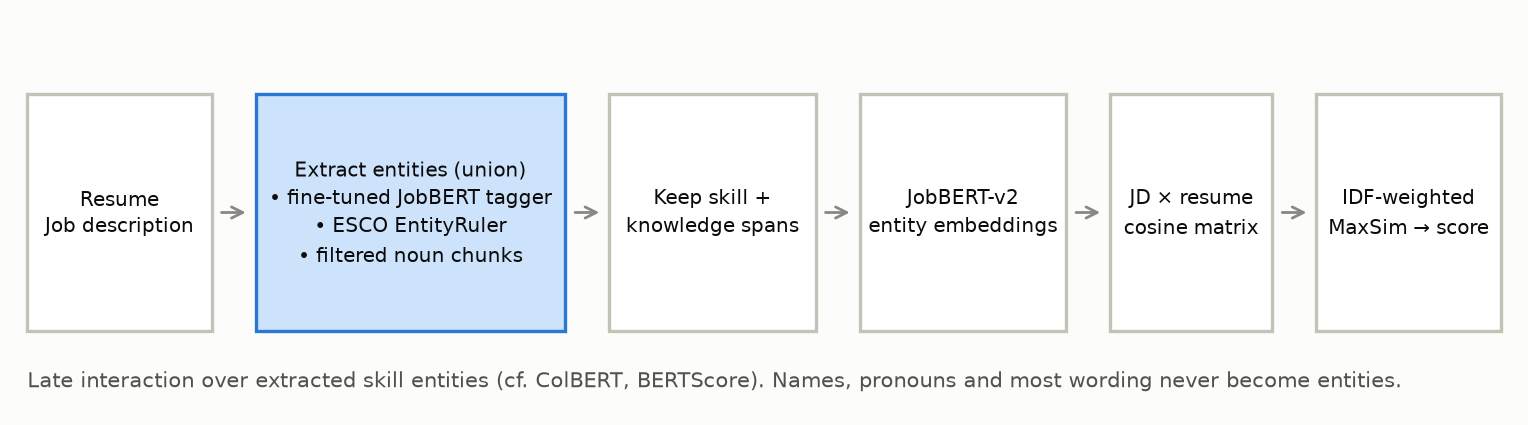
\includegraphics[width=0.9\textwidth]{figs/report_pipeline.png}
\caption{The final method. Only the highlighted step decides what text can influence the score.}
\label{fig:1}
\end{figure*}
\begin{table*}[!t]
\caption{Project Phases}
\label{tab:2}
\centering
\footnotesize
\begin{tabularx}{\textwidth}{c>{\raggedright\arraybackslash}X>{\raggedright\arraybackslash}X}
\hline
\textbf{Phase} & \textbf{Work} & \textbf{Main output} \\
\hline
0 & Audit of the existing app; research scaffolding & \texttt{BACKEND\_\allowbreak{}AUDIT.\allowbreak{}md}, config/seed/cache/provenance modules \\
1 & Skill extractors, SkillSpan evaluation, fine-tuning & 4 extractors, 3 trained tagger seeds \\
2 & BiasBios, job postings, occupation map, relevance, pools & 334 job pools of 100 candidates \\
3 & Eight matchers behind one interface & \texttt{Scorer} protocol, parity test with the old app \\
4 & Counterfactual perturbations & 7 conditions, every substitution logged \\
5 & Metrics, statistics, experiment harness & tie-aware metrics, bootstrap, permutation tests \\
6 & Ablations and near-miss band sweep & 4 ablations, new suggestion band \\
7 & Human annotation tool & Streamlit app, 250-pair stratified sample \\
8 & Final selection, full runs, figures, tables, web app & results in Sections V-A to V-D, deployed application \\
\hline
\end{tabularx}
\end{table*}
\subsection{Audit of the Baseline System}
Before changing anything we read and ran the existing matcher and wrote down exactly what it did.

\subsubsection{How it scored} It extracted ``entities'' from each text with spaCy (\texttt{en\_\allowbreak{}core\_\allowbreak{}web\_\allowbreak{}sm}): named entities of type ORG, PRODUCT, GPE and WORK\_OF\_ART, every noun chunk of 3–59 characters, and short verb phrases. It embedded each entity on its own with \texttt{all-\allowbreak{}MiniLM-\allowbreak{}L6-\allowbreak{}v2}, built the job $\times$ resume cosine matrix, and took each job entity's best match. The score was the share of job entities whose best match reached 0.55. Entities between 0.35 and 0.55 became ``consider reframing'' suggestions.

\subsubsection{What we found} 

\begin{itemize}
\item \textbf{Gendered tokens became skills.} The pronoun ``She'' passed the noun-chunk filter. So did ``Women'' (from ``Women in Tech''), hospital names and cities. The matcher that was supposed to compare skills had a direct path for demographic cues.
\item \textbf{The endpoint was broken.} \texttt{POST /\allowbreak{}analysis/\allowbreak{}match} returned HTTP 500 because the service's output keys no longer matched the response schema. There were no backend tests.
\item \textbf{Nothing was configurable.} Fifteen magic numbers were hardcoded, including both thresholds.
\item \textbf{Outputs were not reproducible.} Entities came from an unordered set, so their order changed between runs.
\item \textbf{The bias checker had bugs.} A masculine score of exactly 1.0 was labelled feminine-coded; hyphenated entries such as ``self-reliant'' could never match; prefix matching flagged ``committee'' for ``commit'' and ``kindergarten'' for ``kind''.
\end{itemize}
The first finding became the motivation for the paper. We kept this matcher, reproduced exactly, as a baseline called \texttt{backend\_\allowbreak{}match}; a test checks that the reproduction returns the same score as the original code. We fixed the 500 error immediately and added endpoint tests.

\subsection{Reproducibility Framework}
We agreed a set of ground rules before writing research code and held to them throughout.

\begin{table*}[!t]
\caption{Ground Rules and Their Implementation}
\label{tab:3}
\centering
\footnotesize
\begin{tabularx}{\textwidth}{>{\raggedright\arraybackslash}X>{\raggedright\arraybackslash}X}
\hline
\textbf{Rule} & \textbf{How it is implemented} \\
\hline
Never fabricate data or numbers & If a dataset could not be downloaded, work stopped until it was supplied manually (ESCO and the LinkedIn postings were). No synthetic stand-ins. \\
Every hyperparameter in config & YAML files under \texttt{research/\allowbreak{}configs/\allowbreak{}}, with \texttt{base:} inheritance and \texttt{-\allowbreak{}-\allowbreak{}set key=value} overrides \\
Seeds everywhere & One seed (13) in \texttt{base.\allowbreak{}yaml}; seeded NumPy generators for sampling, bootstrap and permutation tests \\
Provenance & Every run writes \texttt{run\_\allowbreak{}meta.\allowbreak{}json}: config, git commit, dirty flag, package versions \\
Pinned dependencies & \texttt{research/\allowbreak{}requirements.\allowbreak{}txt} with exact versions \\
Tests on tiny fixtures & 236 fast tests and 8 slow (model-loading) tests for research; 13 fast and 2 slow for the backend \\
Caching & Embeddings, extracted spans and pair scores cached on disk, keyed by model or extractor fingerprint and text hash \\
Quick runs & Every experiment accepts \texttt{-\allowbreak{}-\allowbreak{}subset N} \\
No order dependence & String sets are sorted before use, because Python randomises string hashing per process \\
Verify model IDs & Every Hugging Face model and dataset ID was checked to exist and pinned to a revision \\
\hline
\end{tabularx}
\end{table*}
\subsubsection{Code layout} All research code lives in \texttt{research/\allowbreak{}}: \texttt{common/\allowbreak{}} (config, seeding, provenance, caches), \texttt{extraction/\allowbreak{}}, \texttt{data/\allowbreak{}}, \texttt{scorers/\allowbreak{}}, \texttt{perturbations/\allowbreak{}}, \texttt{metrics/\allowbreak{}}, \texttt{experiments/\allowbreak{}} (runnable scripts), \texttt{annotation/\allowbreak{}}, \texttt{analysis/\allowbreak{}} (figures and tables) and \texttt{tests/\allowbreak{}}.

\subsubsection{Environment} Python 3.14, PyTorch 2.13 with CUDA on an NVIDIA RTX 2060 (6 GB), mixed precision where configured. On CPU, fine-tuning took about two hours per epoch; on the GPU, about 1.5 minutes. The full main experiment takes 1.5–2 hours with warm caches.

\subsubsection{Discipline about splits} Development data is used for every choice: thresholds, the suggestion band, the configuration of the final method. Test data is used only for reporting. Where that discipline was imperfect, Section V-F says so.

\subsection{Skill Extraction and Model Training}
The extractor is the gate that decides what the matcher can see, so we built four and measured them before trusting any.

\subsubsection{The extractors} All share one interface and return typed spans (label: skill, knowledge or verb phrase; source: ESCO, noun chunk, NER, verb or model).

\begin{table*}[!t]
\caption{Skill Extractors}
\label{tab:4}
\centering
\footnotesize
\begin{tabularx}{\textwidth}{l>{\raggedright\arraybackslash}X>{\raggedright\arraybackslash}X}
\hline
\textbf{} & \textbf{Extractor} & \textbf{How it works} \\
\hline
(a) & Noun chunks & A faithful port of the old app's extraction; a parity test checks it returns the same strings \\
(b) & ESCO EntityRuler & spaCy EntityRuler built from ESCO v1.2.1 preferred and alternative labels, matched on lemma and on lower-cased form; each span carries its ESCO concept URI \\
(c) & ESCO + filtered noun chunks & (b) plus noun chunks after a filter that trims determiners, pronouns and stop-words, and drops chunks with no noun or with a generic head (``experience'', ``team'', ``role''\ldots{}) \\
(d) & Fine-tuned JobBERT & Token classifier trained on SkillSpan (below) \\
\hline
\end{tabularx}
\end{table*}
The generic-noun stoplist for (c) was written before looking at any evaluation number.

\subsubsection{Evaluation} We scored each extractor on SkillSpan with exact-match and partial-match span F1. Rule-based extractors stay below 0.2 exact F1. Their recall is reasonable but precision is poor: the old app's noun chunks recover 23\% of gold spans on dev at 4\% precision.

\begin{figure}[!t]
\centering
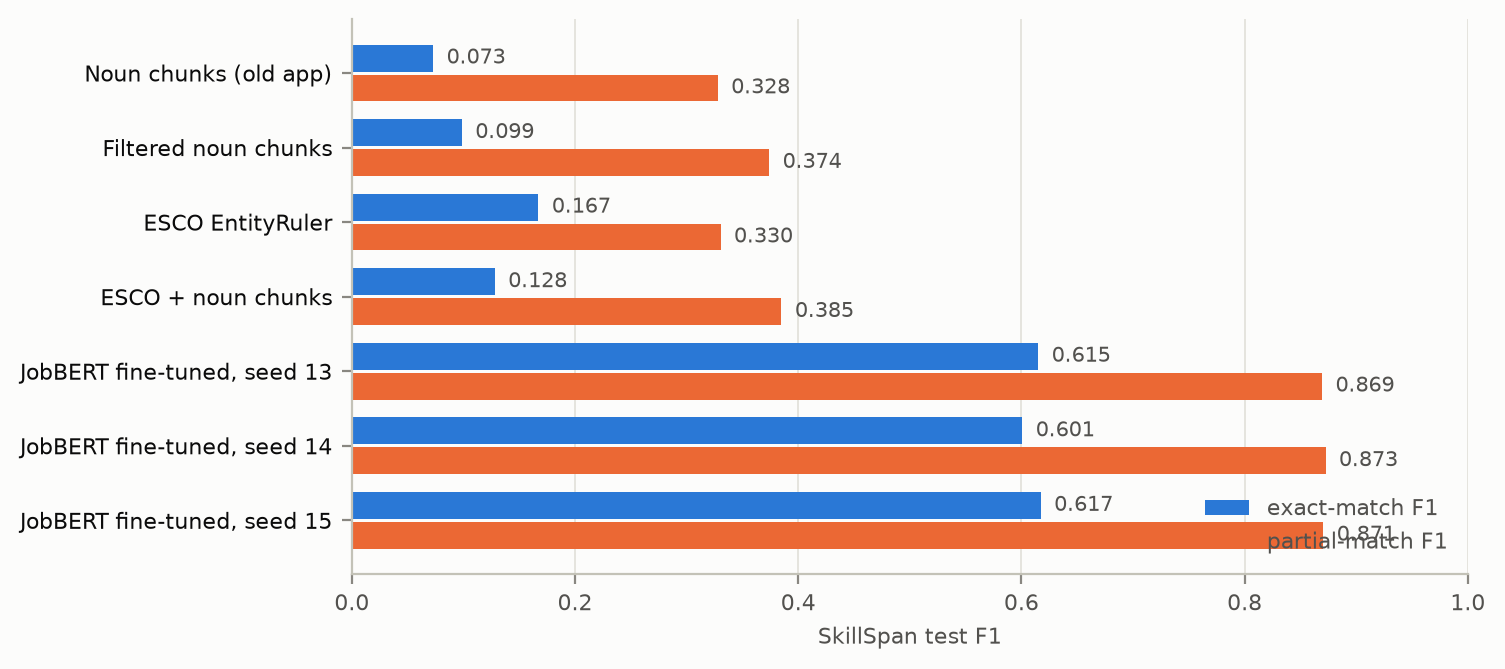
\includegraphics[width=\columnwidth]{figs/report_extraction_f1.png}
\caption{SkillSpan test F1. Only the fine-tuned tagger clears 0.4 exact F1.}
\label{fig:2}
\end{figure}
\begin{table}[!t]
\caption{Extraction Results on the SkillSpan Test Set}
\label{tab:5}
\centering
\footnotesize
\begin{tabularx}{\columnwidth}{>{\raggedright\arraybackslash}X>{\centering\arraybackslash}X>{\centering\arraybackslash}X}
\hline
\textbf{Extractor} & \textbf{Test exact F1} & \textbf{Test partial F1} \\
\hline
Noun chunks (old app) & 0.073 & 0.328 \\
Filtered noun chunks & 0.099 & 0.374 \\
ESCO EntityRuler & 0.167 & 0.330 \\
ESCO + filtered noun chunks & 0.128 & 0.385 \\
Fine-tuned JobBERT (mean of 3 seeds) & 0.611 $\pm$ 0.009 & 0.871 $\pm$ 0.002 \\
\hline
\end{tabularx}
\end{table}
\subsubsection{Fine-tuning} The base model is \texttt{jjzha/\allowbreak{}jobbert-\allowbreak{}base-\allowbreak{}cased}, BERT further pretrained on job postings by the SkillSpan authors. We added one O/B/I classification head per SkillSpan layer (skill, knowledge) over a shared encoder, labelling the first sub-token of each word.

\begin{table}[!t]
\caption{Fine-Tuning Settings}
\label{tab:6}
\centering
\footnotesize
\begin{tabularx}{\columnwidth}{l>{\raggedright\arraybackslash}X}
\hline
\textbf{Setting} & \textbf{Value} \\
\hline
Learning rate & 5e-5, linear warm-up over 10\% of steps \\
Batch size & 16 (evaluation 64) \\
Weight decay / dropout & 0.01 / 0.1 \\
Gradient clipping & 1.0 \\
Max length & 256 sub-tokens (covers the 99th percentile of training sentences) \\
Epochs & up to 10, early stopping after 3 epochs without improvement \\
Model selection & best dev exact span F1 \\
Precision & fp16 mixed precision on CUDA \\
Seeds & 13, 14, 15 \\
\hline
\end{tabularx}
\end{table}
\begin{figure*}[!t]
\centering
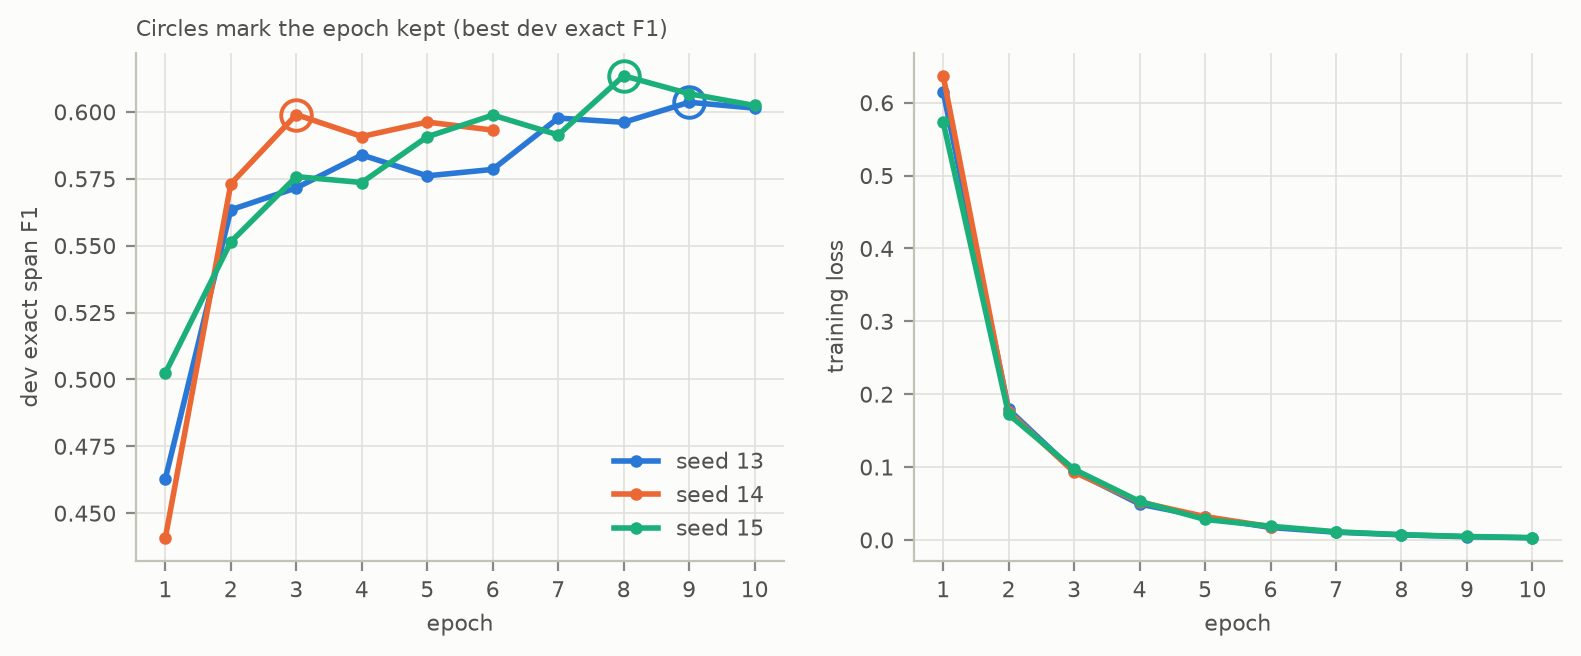
\includegraphics[width=0.9\textwidth]{figs/report_training_curves.png}
\caption{Training curves. Loss falls from about 0.6 to near zero within ten epochs; dev F1 plateaus near 0.60 after epoch 3. Seed 14 stopped early at epoch 6.}
\label{fig:3}
\end{figure*}
\begin{table}[!t]
\caption{Fine-Tuned Tagger Results by Seed}
\label{tab:7}
\centering
\footnotesize
\begin{tabularx}{\columnwidth}{c>{\centering\arraybackslash}X>{\centering\arraybackslash}X>{\centering\arraybackslash}X>{\centering\arraybackslash}X}
\hline
\textbf{Seed} & \textbf{Kept epoch} & \textbf{Dev exact F1} & \textbf{Test exact F1} & \textbf{Test partial F1} \\
\hline
13 & 9 & 0.604 & 0.615 & 0.869 \\
14 & 3 & 0.599 & 0.601 & 0.872 \\
15 & 8 & 0.613 & 0.617 & 0.871 \\
\hline
\end{tabularx}
\end{table}
The three seeds agree to within 0.016 exact F1, so results do not hinge on one lucky run. Downstream experiments use seed 13.

\subsubsection{Error analysis (dev only)} Three observations shaped later decisions.

\begin{itemize}
\item 44\% of ESCO predictions fall in sentences SkillSpan left unannotated, such as titles and tag lines, so its precision is understated.
\item ESCO lacks modern tools: AWS, Docker, React and Kubernetes are not in it.
\item ESCO matches agentic words such as ``lead'' and ``leading'' as skills. This predicted the agentic/communal result in Section V-B.
\end{itemize}
\subsubsection{A training-time obstacle} The first attempt ran on CPU at about two hours per epoch because of the CPU-only PyTorch build and background load. We installed the CUDA build, after which an epoch took about 90 seconds.

\subsection{Datasets and Evaluation Pools}
No public dataset pairs real resumes with job descriptions and demographic labels. We built an evaluation set from two public sources and state its limits plainly.

\subsubsection{Candidates: BiasBios} We used \texttt{LabHC/\allowbreak{}bias\_\allowbreak{}in\_\allowbreak{}bios} (MIT licence, pinned revision), which gives each biography with its first sentence removed, one of 28 occupations and a binary gender label. We kept the official splits and removed in-split duplicates and any dev or test text already seen in an earlier split.

\begin{table}[!t]
\caption{BiasBios Splits After Cleaning}
\label{tab:8}
\centering
\footnotesize
\begin{tabularx}{\columnwidth}{lccc>{\centering\arraybackslash}X}
\hline
\textbf{Split} & \textbf{Raw} & \textbf{Kept} & \textbf{\% female} & \textbf{Mean words} \\
\hline
Train & 257,478 & 257,094 & 46.1 & 60.7 \\
Dev & 39,642 & 39,536 & 46.1 & 60.6 \\
Test & 99,069 & 98,748 & 46.1 & 60.7 \\
\hline
\end{tabularx}
\end{table}
Train bios are used only to fit corpus statistics for the lexical baselines. They are never scored.

\subsubsection{Jobs: LinkedIn postings} The Kaggle \texttt{arshkon/\allowbreak{}linkedin-\allowbreak{}job-\allowbreak{}postings} set (CC BY-SA 4.0) has 123,849 postings. After removing 1,263 that were too short and 16,253 duplicate descriptions, 106,326 remained.

\subsubsection{Mapping postings to occupations} We wrote title patterns and SOC 2018 codes for all 28 occupations before looking at the posting data. Each pattern has include, weak, flag and exclude rules. 8,003 distinct titles matched; 6,889 mapped automatically and 1,114 ambiguous titles were set aside for human review and excluded. Inspecting titles (before running any matcher) led to documented revisions:

\begin{itemize}
\item Most ``architect'' titles were IT roles (solutions architect, data architect), so that occupation also requires architecture-practice terms in the description (Revit, building codes, construction documents and similar).
\item ``Nurse practitioner'' was being auto-mapped to nurse and is now flagged for review.
\item Volunteer, speaker, veterinary and sales-associate titles were excluded globally, and ``DDS'' was demoted to ambiguous for dentist because it also abbreviates a government department.
\end{itemize}
Up to 20 postings per occupation were sampled, giving 334 job descriptions (mean 473 words). Eighteen occupations have pools. Ten had too few postings: comedian, composer, DJ, filmmaker, model, painter, pastor, poet, rapper and yoga teacher. Their bios still appear as irrelevant candidates. Chiropractor (7), surgeon (13) and photographer (14) have fewer than 20 postings.

\subsubsection{Relevance labels} A bio is relevant to a job if it has the same occupation (binary). Graded relevance is 2 for the same occupation, 1 for the same SOC major group (for example physician and nurse) and 0 otherwise.

\subsubsection{Candidate pools} Each job description gets a pool of 100 bios from the matching split:

\begin{itemize}
\item 10 relevant: 5 women and 5 men.
\item 90 irrelevant: 45 women and 45 men, with the occupation drawn uniformly so large occupations do not dominate.
\end{itemize}
Gender balance within each pool means that any difference in how women and men are ranked comes from the matcher, not from base rates. Jobs were split 30/70 into 100 dev pools and 234 test pools. The test pools contain 16,217 distinct bios.

\subsubsection{The honest limitation} A 60-word third-person biography is not a resume. It mentions credentials and employers more than skills, which matters for an entity-based method (Section IV-E) and is discussed in Section V-F.

\subsection{Matching Models}
Every matcher implements one \texttt{Scorer} protocol (\texttt{score(resume, jd)} and \texttt{score\_\allowbreak{}batch(pairs)}) and is built from \texttt{configs/\allowbreak{}scorers.\allowbreak{}yaml}, so all of them run through the same harness, caches and metrics.

\begin{table*}[!t]
\caption{Matchers Compared}
\label{tab:9}
\centering
\footnotesize
\begin{tabularx}{\textwidth}{ll>{\raggedright\arraybackslash}X}
\hline
\textbf{Matcher} & \textbf{Family} & \textbf{What it compares} \\
\hline
BM25 & Lexical & Okapi BM25 over words (k1 = 1.5, b = 0.75), stop-words removed \\
TF-IDF & Lexical & TF-IDF cosine with sublinear term frequency \\
MiniLM & Full-text neural & \texttt{all-\allowbreak{}MiniLM-\allowbreak{}L6-\allowbreak{}v2} embedding of the whole text \\
MPNet & Full-text neural & \texttt{all-\allowbreak{}mpnet-\allowbreak{}base-\allowbreak{}v2} embedding of the whole text \\
JobBERT-v2 & Full-text neural & \texttt{TechWolf/\allowbreak{}JobBERT-\allowbreak{}v2} embedding of the whole text \\
Cross-encoder & Full-text neural & \texttt{ms-\allowbreak{}marco-\allowbreak{}MiniLM-\allowbreak{}L6-\allowbreak{}v2} reading resume and job together \\
Old app matcher & Legacy & The original application, reproduced exactly (Section IV-A) \\
\textbf{Entity LI (ours)} & Entity-level & Skill entities, JobBERT-v2 entity embeddings, IDF-weighted MaxSim \\
\hline
\end{tabularx}
\end{table*}
An LLM-judge baseline (Qwen2.5-1.5B-Instruct) is implemented but was not run; it is too slow for the roughly 267,000 pair scores each matcher needs on this hardware.

\subsubsection{Implementation details that affect the results} 

\begin{itemize}
\item \textbf{Lexical scorers use fixed corpus statistics.} IDF is fitted once on 50,000 train bios plus the pool job descriptions, so a perturbed, unseen resume is scored with the same weights as the original. We re-implemented the BM25Okapi formula for this, and a test checks equality with the \texttt{rank\_\allowbreak{}bm25} library.
\item \textbf{Lexical scorers cannot see pronouns.} The standard English stop-word list removes he, she, his and her. This is why they are almost perfectly invariant to pronoun swaps, and it is a property of the method, not an achievement.
\item \textbf{Long texts are chunked.} Job descriptions average 473 words, beyond the encoders' windows (MiniLM 256 tokens, MPNet 384, JobBERT-v2 64). Full-text scorers split the text into consecutive token windows, embed each, average and renormalise, so every part of the text counts.
\item \textbf{JobBERT-v2 is used outside its design.} It was trained on job titles and skill lists, not documents. We use it on 64-token windows and state this as a limitation.
\end{itemize}
\subsubsection{Our scorer} Given a resume and a job description:

\begin{enumerate}
\item Extract typed spans from both texts.
\item Keep spans labelled skill or knowledge; deduplicate case-insensitively.
\item Embed each distinct entity string on its own.
\item Build the job $\times$ resume cosine-similarity matrix S.
\item Aggregate. For each job entity take its best resume match, then take the IDF-weighted mean:
\end{enumerate}
\begin{equation}
\mathrm{score}(r, j) = \sum_{i \in E_j} \frac{\mathrm{idf}(i)}{\sum_{k \in E_j} \mathrm{idf}(k)} \, \max_{m \in E_r} \cos(\mathbf{e}_i, \mathbf{e}_m)
\end{equation}
\begin{equation}
\mathrm{idf}(e) = \ln\frac{N + 1}{\mathrm{df}(e) + 1} + 1
\end{equation}
Here $E_j$ and $E_r$ are the entity sets of the job and the resume, and document frequency is counted over the N = 334 job descriptions. The score is recall-oriented: it asks how well the resume covers what the job asks for. Four aggregations are implemented (MaxSim mean, IDF-weighted MaxSim, Hungarian one-to-one assignment, and the old app's threshold fraction).

\subsubsection{The key risk we found on dev} Our first version used only the fine-tuned tagger and ESCO. On BiasBios, the tagger finds no skill entity in about half of all bios, because bios list credentials and employers, not skills. A pair with no entities scores 0 before and after any rewrite, which looks like perfect fairness for a trivial reason. On 30 dev pools that version left 23\% of pairs empty and reached AUC 0.68 against 0.81 for full-text MiniLM.

We responded in two ways. First, every result reports the share of pairs with entities on both sides, and entity scorers also report gaps restricted to those pairs. Second, the ablation in Section V-B showed that adding filtered noun chunks restores coverage to 100\% and improves accuracy, which led to the final method (Section V-C).

\subsection{Counterfactual Perturbation Design}
Each bio is parsed once with spaCy. Independent ``parts'' propose token-range replacements, and a condition merges one or more parts. Every substitution is logged with its original text, replacement and character offsets, so any counterfactual can be inspected.

\begin{table*}[!t]
\caption{Counterfactual Conditions}
\label{tab:10}
\centering
\footnotesize
\begin{tabularx}{\textwidth}{>{\raggedright\arraybackslash}X>{\raggedright\arraybackslash}Xl}
\hline
\textbf{Condition} & \textbf{What changes} & \textbf{Cue tested} \\
\hline
Pronoun swap & he $\leftrightarrow$ she, him/his $\leftrightarrow$ her, himself $\leftrightarrow$ herself, Mr $\leftrightarrow$ Ms & Gender (pronouns) \\
Name swap (US) & Subject's first name $\rightarrow$ a US name of the other gender & Gender (name) \\
Name swap (Indian) & Subject's first name $\rightarrow$ an Indian name of the other gender & Gender + ethnicity \\
Indian name, same gender & Subject's first name $\rightarrow$ an Indian name of the same gender & Ethnicity only \\
Affiliation swap & Gendered affiliations (e.g. women's college $\leftrightarrow$ men's) & Gender (affiliation) \\
Agentic $\rightarrow$ communal & Agentic wording $\rightarrow$ communal (e.g. led $\rightarrow$ supported) & Gendered style \\
Full gender flip & Pronoun swap + US name swap & Gender (complete) \\
\hline
\end{tabularx}
\end{table*}
\subsubsection{Making the rewrites correct was most of the work} We sampled 50 rewrites per condition into a review file, inspected them and fixed what was wrong. A full human review of that file is still pending. The guards that resulted:

\begin{itemize}
\item \textbf{Pronouns.} ``her'' is ambiguous. It becomes ``his'' when tagged as a possessive (``her lab'') and ``him'' as an object (``taught her''); when the tag is unclear, the next token decides.
\item \textbf{Whose name?} Early versions swapped any first name, including other people's (``roasts of Bob Saget''). Now a name is swapped only if it is a strongly gendered first name (at least 95\% one gender), matches the bio's gender, does not follow a title, is not a surname, and looks like the bio's subject (a single-word mention or a clause subject).
\item \textbf{Name sources.} US names come from Social Security Administration national counts: the detection lexicon uses births from 1930–2005, and the replacement pool is the 200 most common names per gender from 1950–2000 that are at least 98\% one gender. Indian names are the 100 most common given names per gender among Indian citizens in Wikidata, excluding names also common in the US. We rejected two candidate name lists: one without gender or provenance, one containing customer data.
\item \textbf{Agentic wording.} Verb swaps are restricted by part of speech and dependency, skip passives, and skip idioms: ``led to'', ``lead the way'', phrasal verbs, hyphenated compounds and verbs whose object is ``way'', ``life'' or ``language''. A rule mapping ``support'' to ``lead'' was removed because it produced false rewrites.
\end{itemize}
\subsubsection{Coverage is uneven by design} A rewrite only applies when there is something to rewrite.

\begin{table}[!t]
\caption{Perturbation Coverage on Test Bios}
\label{tab:11}
\centering
\footnotesize
\begin{tabularx}{\columnwidth}{l>{\centering\arraybackslash}X>{\centering\arraybackslash}X}
\hline
\textbf{Condition} & \textbf{\% of test bios changed} & \textbf{Mean substitutions when changed} \\
\hline
Pronoun swap & 99.0 & 3.09 \\
Name swaps (all three) & 19.5 & 1.60 \\
Affiliation swap & 0.3 & 1.04 \\
Agentic $\rightarrow$ communal & 2.5 & 1.04 \\
Full gender flip & 99.3 & 3.40 \\
\hline
\end{tabularx}
\end{table}
An unchanged bio has an identical counterfactual and a gap of exactly zero. Averaging over all bios would therefore reward conditions that rarely apply. All headline gaps are computed over changed bios only. The affiliation and agentic conditions touch few bios, so their estimates are noisy.

\subsubsection{Examples from the dev split} 

\begin{table*}[!t]
\caption{Example Counterfactuals From the Dev Split}
\label{tab:12}
\centering
\footnotesize
\begin{tabularx}{\textwidth}{l>{\raggedright\arraybackslash}X>{\raggedright\arraybackslash}X}
\hline
\textbf{Condition} & \textbf{Substitutions} & \textbf{Rewritten text (excerpt)} \\
\hline
Full gender flip & He $\rightarrow$ She, Jim $\rightarrow$ Natalie & ``She is a WebSphere Application Server developer\ldots{} Natalie's worked in WebSphere Application Server development for four years.'' \\
Name swap (Indian) & Mike $\rightarrow$ Radhika & ``Radhika began his processional carrier [sic] at IBM, where he became well versed in data warehouse design\ldots{}'' \\
\hline
\end{tabularx}
\end{table*}
The second example shows the design intent: only the name changes, so the pronouns still say ``he''. The condition isolates the name cue.

\subsection{Evaluation Metrics and Statistical Analysis}
\subsubsection{Ranking accuracy} For each pool we compute graded nDCG@10 (gain 2\textasciicircum{}g $-$ 1), binary nDCG@10, MRR, P@5 and P@10. Entity scorers can give many exactly tied scores, and standard implementations break ties by input order, which silently favours or penalises a method. We use tie-aware expected metrics \cite{mcsherry}: the value averaged over all orderings of each tied group, computed in closed form and tested against hand-worked examples.

\subsubsection{Counterfactual gap} For a bio b in the pool of job j, with original score s and counterfactual score s$'$:

\begin{equation}
\mathrm{gap}(b, j) = \frac{\lvert s'(b, j) - s(b, j) \rvert}{\sigma_j}
\end{equation}
where $\sigma_j$ is the SD of the original scores in pool $j$.
Dividing by the pool's standard deviation is essential. BM25 scores run into the tens, cosines sit between 0 and 1, and the old app's score moves in steps. In normalised units, 0.1 means the rewrite moved a candidate by a tenth of the typical spread between candidates for that job. The pool-level statistic is the mean over changed bios.

We also report:

\begin{itemize}
\item \textbf{Signed gap}, oriented so that positive means the female-coded (or communal, or target-name) version scores higher. It shows direction, where the absolute gap shows magnitude.
\item \textbf{Rank shift}: the mean absolute change in a candidate's rank within the 100-candidate pool.
\item \textbf{Non-empty gap}: for entity scorers, the gap restricted to pairs with entities on both sides.
\end{itemize}
\subsubsection{Group metrics} 

\begin{itemize}
\item \textbf{TPR gap.} A threshold is chosen on dev (best F1 on per-pool z-scores) and applied to test. Per occupation we compute the true-positive rate of relevant women minus relevant men, then report the mean and the root mean square across occupations.
\item \textbf{Top-10 exposure.} The female share of the top 10 minus 0.5; pools are 50/50, so parity is zero.
\end{itemize}
\subsubsection{Uncertainty} Pairs sharing a job description are not independent, so the resampling unit is the pool. Confidence intervals are 95\% percentile intervals from a cluster bootstrap over pools (1,000 resamples, seeded).

\subsubsection{Significance} Our matcher is compared with each baseline by a two-sided paired sign-flip permutation test on per-pool differences (10,000 permutations), with Holm correction within each metric family.

\subsubsection{A statistic we report without an interval} The bootstrap interval for the RMS TPR gap excluded its own point estimate: resampling occupations inflates an RMS of small gaps. A basic (reverse-percentile) interval did not fix it. We report the RMS as a point estimate only and give intervals for the mean TPR gap.

\subsubsection{The harness} One script, \texttt{research.\allowbreak{}experiments.\allowbreak{}run}, loads pools and counterfactuals, scores every (matcher, condition) once with caching, writes \texttt{scores.\allowbreak{}parquet}, \texttt{per\_\allowbreak{}pool.\allowbreak{}parquet}, \texttt{metrics.\allowbreak{}csv} and \texttt{tests.\allowbreak{}csv}, and renders a summary. Metrics can be recomputed from stored scores without re-scoring.

\section{Results and Discussion}
\subsection{Main Results}
All numbers are from the full run on 234 test pools: means over pools with 95\% cluster-bootstrap intervals. The entity matcher is the final method chosen in Section V-C.

\subsubsection{The headline} The entity-level matcher sits in the lower right of the accuracy–leakage plane, among the neural matchers on accuracy and near the lexical matchers on leakage.

\begin{figure}[!t]
\centering
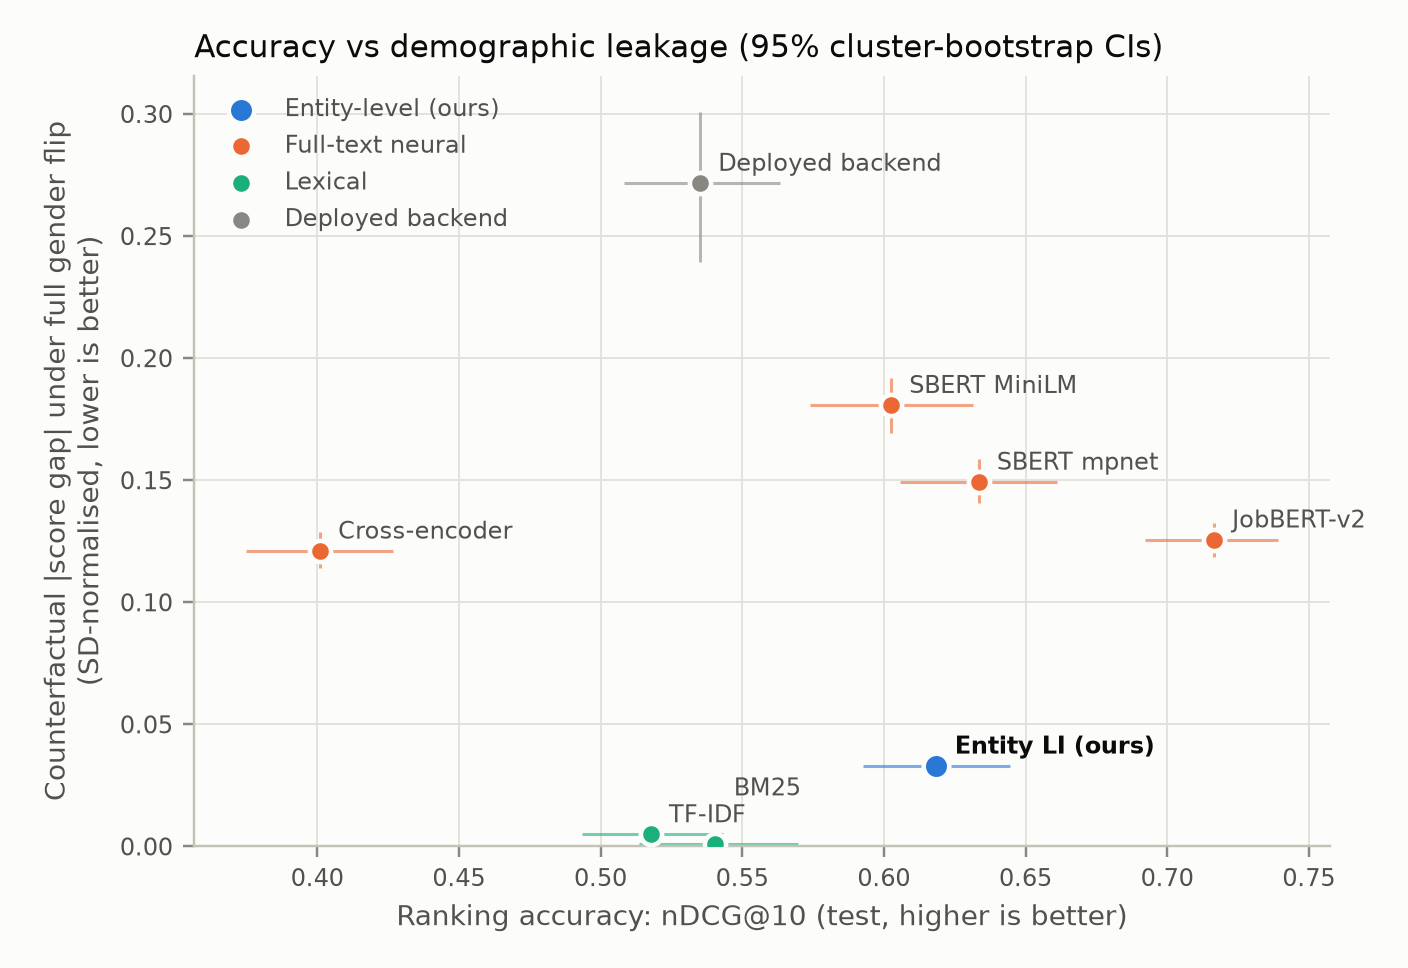
\includegraphics[width=\columnwidth]{figs/headline_accuracy_vs_gap.png}
\caption{nDCG@10 (right is better) against the normalised score change under the full gender flip (down is better). Colour encodes matcher family; bars are 95\% intervals.}
\label{fig:4}
\end{figure}
\subsubsection{RQ2: ranking accuracy} 

\begin{table}[!t]
\caption{Ranking Accuracy on 234 Test Pools}
\label{tab:13}
\centering
\footnotesize
\begin{tabular}{llccc}
\hline
\textbf{Matcher} & \textbf{nDCG@10} & \textbf{MRR} & \textbf{P@5} & \textbf{P@10} \\
\hline
JobBERT-v2 (full text) & 0.716 [0.692, 0.739] & 0.907 & 0.743 & 0.613 \\
MPNet & 0.633 [0.606, 0.661] & 0.859 & 0.650 & 0.535 \\
\textbf{Entity LI (ours)} & \textbf{0.619 [0.592, 0.644]} & 0.843 & 0.641 & 0.518 \\
MiniLM & 0.602 [0.574, 0.631] & 0.836 & 0.635 & 0.498 \\
BM25 & 0.541 [0.514, 0.570] & 0.799 & 0.582 & 0.441 \\
Old app matcher & 0.535 [0.508, 0.563] & 0.793 & 0.552 & 0.438 \\
TF-IDF & 0.518 [0.494, 0.543] & 0.791 & 0.555 & 0.421 \\
Cross-encoder & 0.401 [0.375, 0.427] & 0.657 & 0.407 & 0.322 \\
\hline
\end{tabular}
\end{table}
Our matcher is statistically tied with MiniLM and MPNet (Holm p = 0.39 for both), significantly better than BM25, TF-IDF, the cross-encoder and the old app matcher (p < 0.001), and significantly worse than full-text JobBERT-v2 by 0.098 nDCG (p < 0.001). The cross-encoder's low score is expected: it was trained for web passage ranking, not job matching.

\subsubsection{RQ1: counterfactual leakage} Mean absolute score change in pool SDs, over changed bios.

\begin{table*}[!t]
\caption{Counterfactual Gap by Condition (Pool SDs, Changed Bios)}
\label{tab:14}
\centering
\footnotesize
\begin{tabularx}{\textwidth}{lc>{\centering\arraybackslash}X>{\centering\arraybackslash}X>{\centering\arraybackslash}X>{\centering\arraybackslash}X>{\centering\arraybackslash}X>{\centering\arraybackslash}X}
\hline
\textbf{Matcher} & \textbf{Pronoun} & \textbf{Name (US)} & \textbf{Name (Indian)} & \textbf{Indian name, same gender} & \textbf{Affiliation} & \textbf{Agentic $\rightarrow$ communal} & \textbf{Full gender flip} \\
\hline
BM25 & 0.000 & 0.002 & 0.001 & 0.001 & 0.047 & 0.056 & 0.001 \\
TF-IDF & 0.001 & 0.019 & 0.032 & 0.032 & 0.062 & 0.071 & 0.005 \\
\textbf{Entity LI (ours)} & \textbf{0.022} & \textbf{0.058} & \textbf{0.064} & \textbf{0.058} & \textbf{0.046} & \textbf{0.066} & \textbf{0.033} \\
Cross-encoder & 0.103 & 0.156 & 0.212 & 0.203 & 0.108 & 0.058 & 0.121 \\
JobBERT-v2 & 0.107 & 0.135 & 0.189 & 0.188 & 0.057 & 0.058 & 0.126 \\
MPNet & 0.117 & 0.216 & 0.233 & 0.227 & 0.076 & 0.046 & 0.149 \\
MiniLM & 0.135 & 0.280 & 0.294 & 0.284 & 0.068 & 0.045 & 0.181 \\
Old app matcher & 0.272 & 0.008 & 0.010 & 0.007 & 0.069 & 0.051 & 0.272 \\
\hline
\end{tabularx}
\end{table*}
\begin{figure*}[!t]
\centering
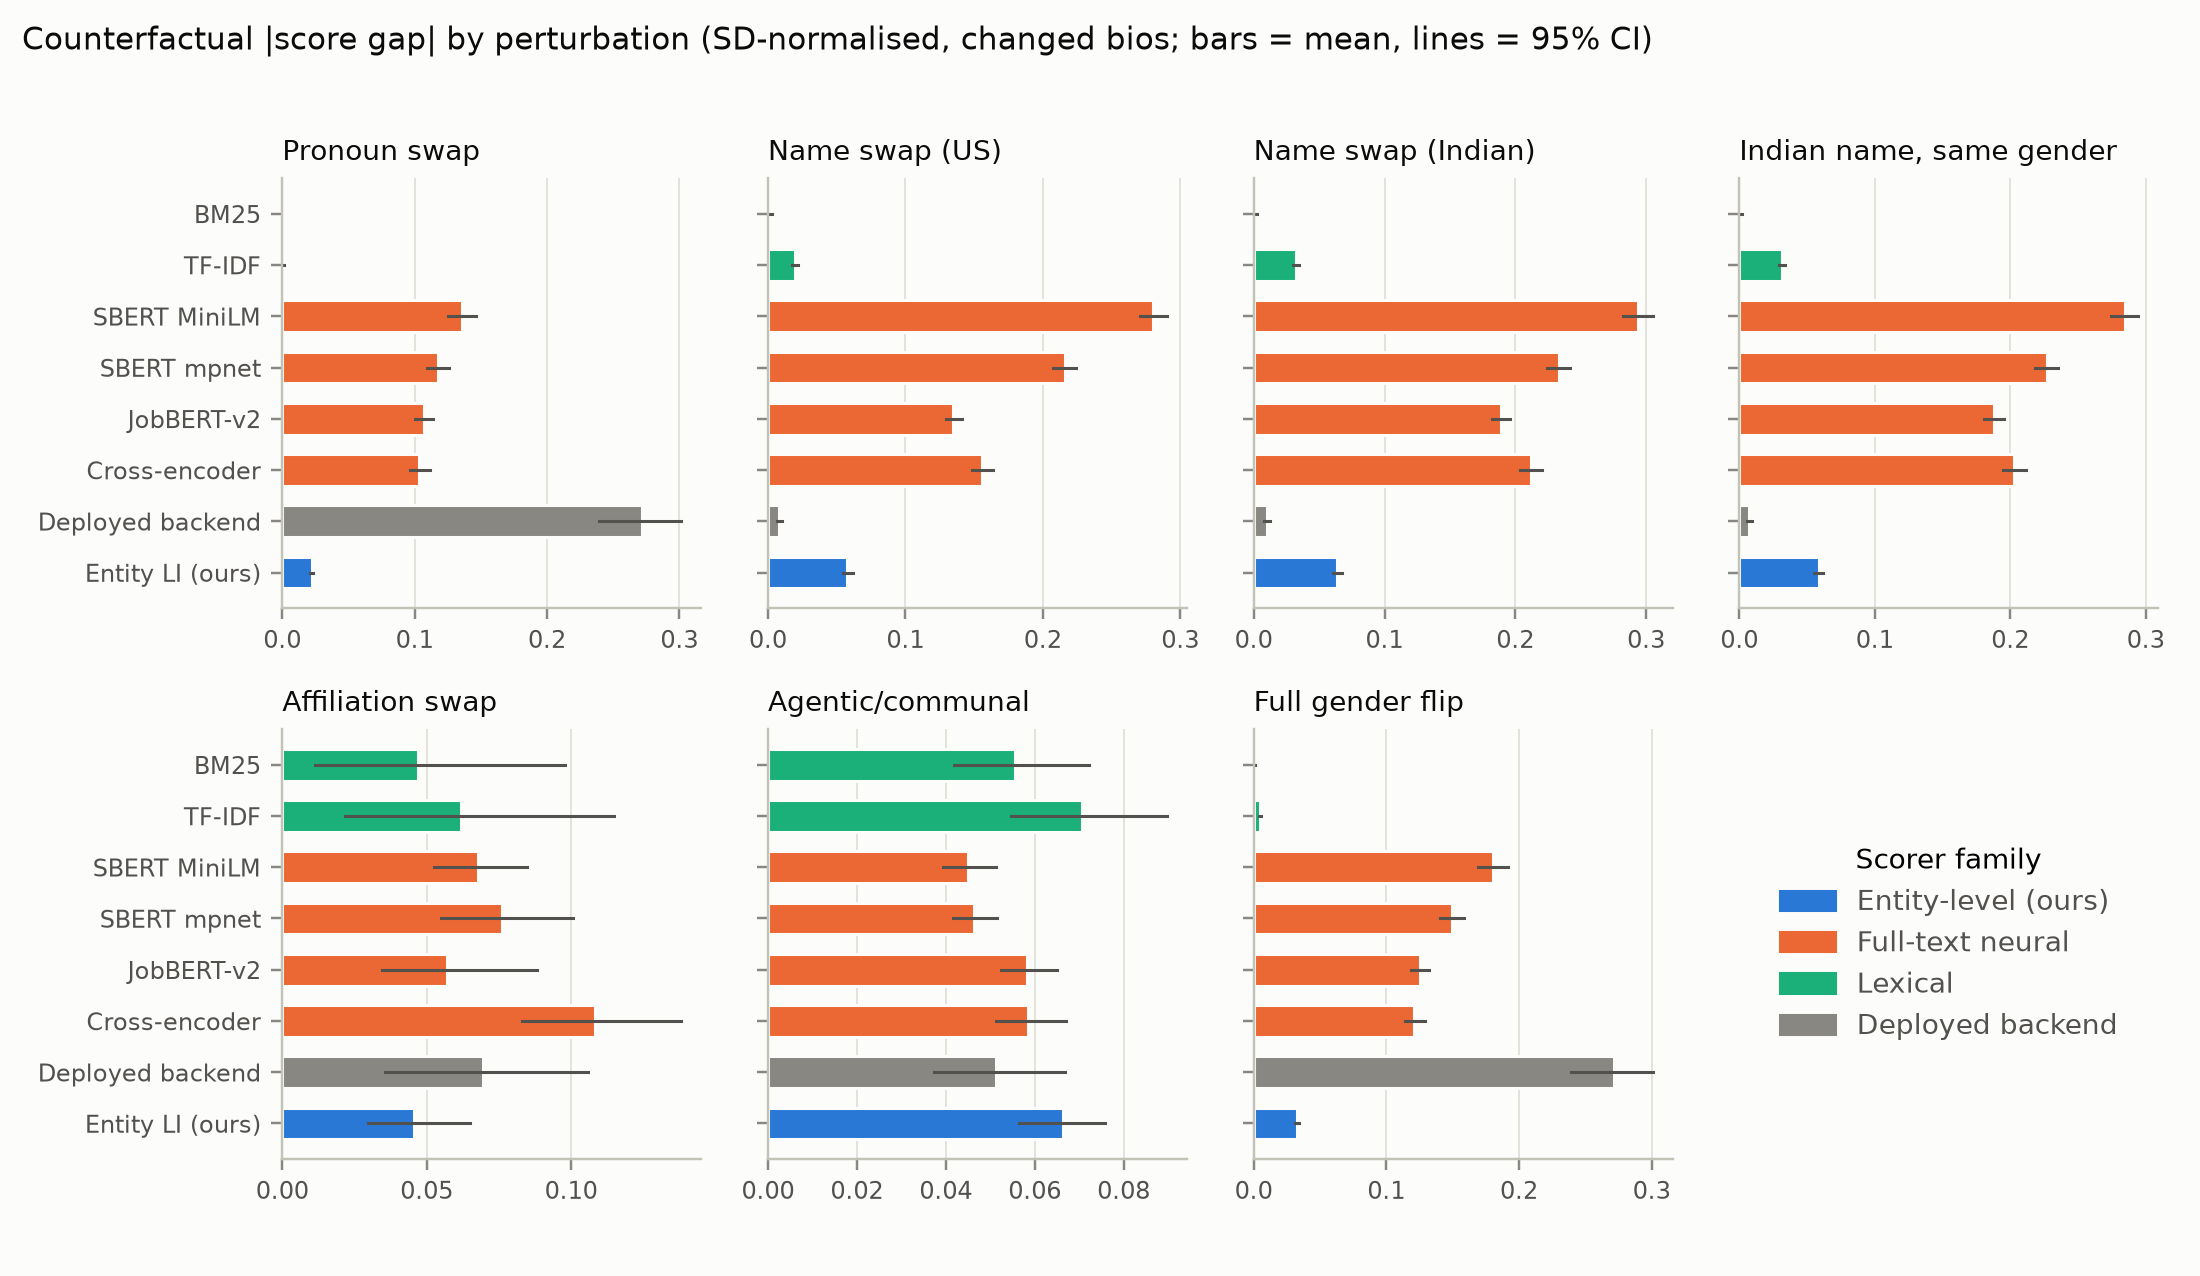
\includegraphics[width=0.9\textwidth]{figs/perturbation_gaps.png}
\caption{The same gaps per perturbation, with 95\% intervals.}
\label{fig:5}
\end{figure*}
What the table shows:

\begin{itemize}
\item \textbf{Against full-text neural matchers the hypothesis holds.} On all four gender and name conditions, and on the full flip, our gap is between a fifth and under a half of the best neural matcher's, and about a fifth of MiniLM's. Every one of these comparisons is significant (Holm p < 0.001).
\item \textbf{Against lexical matchers it does not.} BM25 and TF-IDF move less than we do on pronouns and names (p < 0.001), because they cannot see pronouns at all and treat a name as one rare word among many.
\item \textbf{Names leak more than pronouns for us.} Filtered noun chunks let some names through as entities (0.058 against 0.022).
\item \textbf{The old app matcher is a special case.} It has the largest pronoun gap of all (0.272), because ``She'' and ``He'' were entities for it, and almost none for names.
\item \textbf{Ethnicity cues matter to neural matchers.} Swapping to an Indian name of the same gender moves MiniLM by 0.284, as much as a cross-gender swap. Our matcher moves by 0.058.
\item \textbf{Agentic wording moves everyone alike} (0.045–0.071). We are slightly but significantly above MiniLM and MPNet here (differences of 0.02, p $\le$ 0.002), which the ablations explain.
\item \textbf{The affiliation condition is underpowered.} It changes 0.3\% of bios; only the comparison with the cross-encoder is significant.
\end{itemize}
\subsubsection{Significance, full gender flip} Mean per-pool difference, ours minus baseline (negative means we leak less).

\begin{table}[!t]
\caption{Paired Tests Against Each Baseline, Full Gender Flip}
\label{tab:15}
\centering
\footnotesize
\begin{tabularx}{\columnwidth}{lcc>{\centering\arraybackslash}Xc}
\hline
\textbf{Baseline} & \textbf{$\Delta$ gap} & \textbf{Holm p} & \textbf{$\Delta$ nDCG@10} & \textbf{Holm p} \\
\hline
Old app matcher & $-$0.239 & < 0.001 & +0.083 & < 0.001 \\
MiniLM & $-$0.148 & < 0.001 & +0.016 & 0.39 \\
MPNet & $-$0.116 & < 0.001 & $-$0.015 & 0.39 \\
JobBERT-v2 & $-$0.093 & < 0.001 & $-$0.098 & < 0.001 \\
Cross-encoder & $-$0.088 & < 0.001 & +0.218 & < 0.001 \\
TF-IDF & +0.028 & < 0.001 & +0.101 & < 0.001 \\
BM25 & +0.032 & < 0.001 & +0.078 & < 0.001 \\
\hline
\end{tabularx}
\end{table}
\subsubsection{In ranks} Under the full gender flip, a candidate moves on average 0.98 places in a pool of 100 with our matcher, against 3.7–5.2 places for the neural full-text matchers, 10.1 for the old app matcher and under 0.2 for the lexical ones.

\subsubsection{Direction} The signed gap shows who benefits. MiniLM and MPNet favour the female-coded version (+0.099 and +0.097 pool SDs under the full flip), JobBERT-v2 less so (+0.049), the cross-encoder favours the male-coded version ($-$0.037), and the old app matcher strongly favours the female version (+0.258). Ours is $-$0.005: small, though its interval excludes zero.

\subsubsection{Group metrics} 

\begin{table*}[!t]
\caption{Group Fairness Metrics}
\label{tab:16}
\centering
\footnotesize
\begin{tabularx}{\textwidth}{l>{\raggedright\arraybackslash}X>{\centering\arraybackslash}X>{\raggedright\arraybackslash}X}
\hline
\textbf{Matcher} & \textbf{Mean TPR gap (F $-$ M)} & \textbf{RMS TPR gap} & \textbf{Top-10 female share $-$ 0.5} \\
\hline
BM25 & 0.009 [$-$0.032, 0.046] & 0.131 & 0.019 [$-$0.000, 0.037] \\
TF-IDF & 0.031 [$-$0.009, 0.070] & 0.123 & 0.020 [$-$0.001, 0.038] \\
MiniLM & 0.063 [0.026, 0.102] & 0.136 & 0.063 [0.045, 0.081] \\
MPNet & 0.057 [0.017, 0.101] & 0.134 & 0.059 [0.042, 0.076] \\
JobBERT-v2 & 0.018 [$-$0.021, 0.055] & 0.134 & 0.014 [$-$0.003, 0.030] \\
Cross-encoder & 0.013 [$-$0.022, 0.049] & 0.068 & $-$0.002 [$-$0.023, 0.017] \\
Old app matcher & 0.052 [0.017, 0.090] & 0.120 & 0.082 [0.063, 0.101] \\
\textbf{Entity LI (ours)} & 0.009 [$-$0.030, 0.049] & 0.083 & 0.010 [$-$0.005, 0.026] \\
\hline
\end{tabularx}
\end{table*}
MiniLM, MPNet and the old app matcher over-select women: their mean TPR gap and top-10 share intervals exclude zero. Ours, the lexical matchers, JobBERT-v2 and the cross-encoder are consistent with parity. This agrees with the signed counterfactual gaps, which is reassuring because the two analyses share no machinery.

\subsection{Ablation Study}
Each ablation changes one component of the reference method used in Phases 3–6 (JobBERT + ESCO extractor, skill and knowledge spans only, MiniLM entity embeddings, MaxSim mean) and is run on all 234 test pools. Gaps are in pool SDs over changed bios. ``Pairs with entities'' is the share of pairs with at least one entity on both sides.

\subsubsection{Extractor} (encoder and aggregation fixed).

\begin{table*}[!t]
\caption{Ablation: Extractor}
\label{tab:17}
\centering
\footnotesize
\begin{tabularx}{\textwidth}{>{\raggedright\arraybackslash}Xc>{\centering\arraybackslash}Xc>{\centering\arraybackslash}Xc>{\centering\arraybackslash}X}
\hline
\textbf{Extractor} & \textbf{nDCG@10} & \textbf{Pairs with entities} & \textbf{Pronoun} & \textbf{Name (US)} & \textbf{Agentic} & \textbf{Full flip} \\
\hline
Noun chunks (old app) & 0.477 & 100\% & 0.163 & 0.031 & 0.051 & 0.164 \\
ESCO ruler & 0.378 & 69\% & 0.000 & 0.007 & 0.563 & 0.002 \\
Fine-tuned JobBERT & 0.324 & 37\% & 0.161 & 0.069 & 0.159 & 0.170 \\
JobBERT + ESCO (reference) & 0.441 & 76\% & 0.070 & 0.040 & 0.450 & 0.075 \\
\hline
\end{tabularx}
\end{table*}
This is the clearest finding of the project: \textbf{the extractor decides what leaks.}

\begin{itemize}
\item The ESCO ruler is a dictionary. It cannot react to a pronoun or a name, so its gender gaps are essentially zero. But ``lead'' and ``leading'' are ESCO skills, so rewriting ``led'' as ``supported'' removes an entity, and its agentic gap is the largest in the study (0.563).
\item The fine-tuned tagger is contextual. Swapping ``She'' for ``He'' changes the hidden states of neighbouring tokens, which changes which spans it tags, which changes the score. Its pronoun gap (0.161) is as large as the old app's, even though it never tags a pronoun as a skill. It also finds entities in only 37\% of pairs.
\item Unfiltered noun chunks leak through pronouns directly.
\end{itemize}
A learned extractor is therefore not automatically safer than a dictionary: it is more accurate on SkillSpan and more sensitive to context that should not matter.

\subsubsection{Entity types} (which spans are kept).

\begin{table*}[!t]
\caption{Ablation: Entity Types}
\label{tab:18}
\centering
\footnotesize
\begin{tabularx}{\textwidth}{>{\raggedright\arraybackslash}Xc>{\centering\arraybackslash}Xc>{\centering\arraybackslash}Xc>{\centering\arraybackslash}X}
\hline
\textbf{Entities} & \textbf{nDCG@10} & \textbf{Pairs with entities} & \textbf{Pronoun} & \textbf{Name (US)} & \textbf{Agentic} & \textbf{Full flip} \\
\hline
Skills only (reference) & 0.441 & 76\% & 0.070 & 0.040 & 0.450 & 0.075 \\
+ filtered noun chunks & 0.546 & 100\% & 0.026 & 0.036 & 0.151 & 0.033 \\
+ noun chunks + verb phrases & 0.524 & 100\% & 0.026 & 0.034 & 0.122 & 0.032 \\
\hline
\end{tabularx}
\end{table*}
We expected more entity types to let more demographic signal in. The opposite happened. Filtered noun chunks raise nDCG by 0.105, fill every empty pair, and cut every gap. The likely reason is dilution: with more entities per text, a single changed span has less weight. Verb phrases add nothing to accuracy.

\subsubsection{Entity encoder} 

\begin{table}[!t]
\caption{Ablation: Entity Encoder}
\label{tab:19}
\centering
\footnotesize
\begin{tabularx}{\columnwidth}{lcc>{\centering\arraybackslash}Xc>{\centering\arraybackslash}X}
\hline
\textbf{Encoder} & \textbf{nDCG@10} & \textbf{Pronoun} & \textbf{Name (US)} & \textbf{Agentic} & \textbf{Full flip} \\
\hline
MiniLM (reference) & 0.441 & 0.070 & 0.040 & 0.450 & 0.075 \\
MPNet & 0.433 & 0.067 & 0.040 & 0.373 & 0.073 \\
JobBERT-v2 & 0.486 & 0.061 & 0.041 & 0.281 & 0.067 \\
\hline
\end{tabularx}
\end{table}
JobBERT-v2, trained on short title and skill strings, is the best encoder for entities: more accurate and less sensitive to agentic wording. The encoder barely affects gender gaps.

\subsubsection{Aggregation} 

\begin{table}[!t]
\caption{Ablation: Aggregation}
\label{tab:20}
\centering
\footnotesize
\begin{tabularx}{\columnwidth}{>{\raggedright\arraybackslash}Xcc>{\centering\arraybackslash}Xc>{\centering\arraybackslash}X}
\hline
\textbf{Aggregation} & \textbf{nDCG@10} & \textbf{Pronoun} & \textbf{Name (US)} & \textbf{Agentic} & \textbf{Full flip} \\
\hline
MaxSim mean (reference) & 0.441 & 0.070 & 0.040 & 0.450 & 0.075 \\
Hungarian (one-to-one) & 0.267 & 0.101 & 0.052 & 0.447 & 0.109 \\
IDF-weighted MaxSim & 0.452 & 0.070 & 0.040 & 0.439 & 0.075 \\
\hline
\end{tabularx}
\end{table}
One-to-one assignment is much worse: a short bio has fewer entities than a long posting, so most job entities go unassigned. IDF weighting helps accuracy slightly and leaves fairness unchanged.

\subsubsection{Answer to RQ3} The extractor and the set of entity types control leakage. The encoder and the aggregation mainly affect accuracy.

\subsection{Model Selection and Held-Out Validation}
\subsubsection{The decision} After the ablations we had a reference method with a known weakness (24\% of pairs empty, nDCG 0.441) and evidence that noun chunks and JobBERT-v2 would help. Two paths were open: report the reference method as it was, or select a better configuration properly. We chose to select, under a rule written down before running anything.

\subsubsection{The rule} (\texttt{configs/\allowbreak{}selection.\allowbreak{}yaml}): score every candidate on the 100 dev pools only; pick the highest dev nDCG@10; break ties within 0.005 in favour of the simpler variant. Fairness metrics are not consulted, because they are the outcome under test.

\subsubsection{The candidates} Two extractor unions (JobBERT + ESCO + filtered noun chunks; ESCO + filtered noun chunks) $\times$ two entity encoders (MiniLM, JobBERT-v2) $\times$ two aggregations (MaxSim mean, IDF-weighted).

\begin{figure}[!t]
\centering
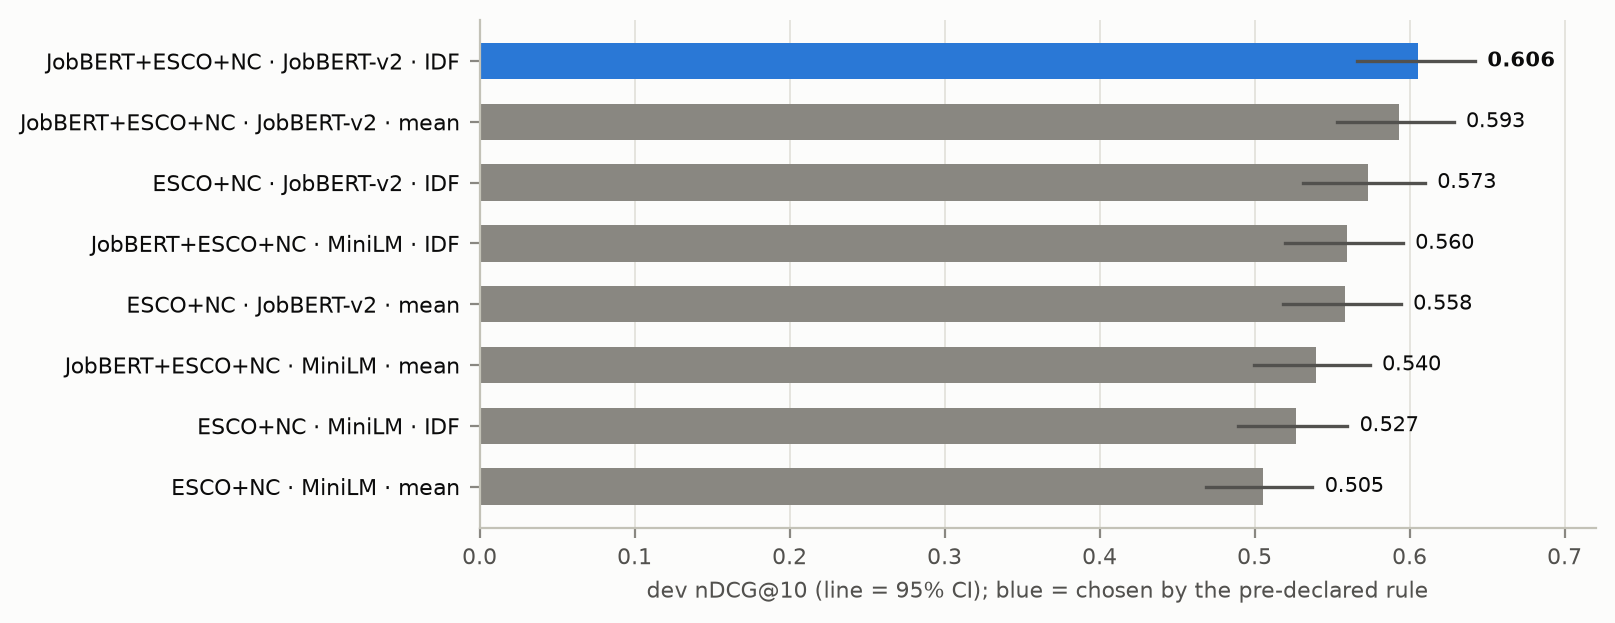
\includegraphics[width=\columnwidth]{figs/report_selection_dev.png}
\caption{Dev-only selection. Each factor helps independently: the three-way union, JobBERT-v2, and IDF weighting.}
\label{fig:6}
\end{figure}
\subsubsection{The final method} is the top row: union of the fine-tuned JobBERT tagger (seed 13), the ESCO ruler and filtered noun chunks; skill and knowledge spans; JobBERT-v2 entity embeddings; IDF-weighted MaxSim. Dev nDCG@10 is 0.606, and test nDCG@10 is 0.619. It finds entities in every test pair.

\subsubsection{The weakness in this procedure, and the check} The candidate family was motivated by ablations that had been run on 200 of the 234 test pools. The final choice among candidates used dev only, but the idea of which candidates to try was informed by test data. That is a form of leakage, and we report it.

The remaining 34 test pools had never been scored by anything before the final run. They give a clean check of the whole design loop.

\begin{figure}[!t]
\centering
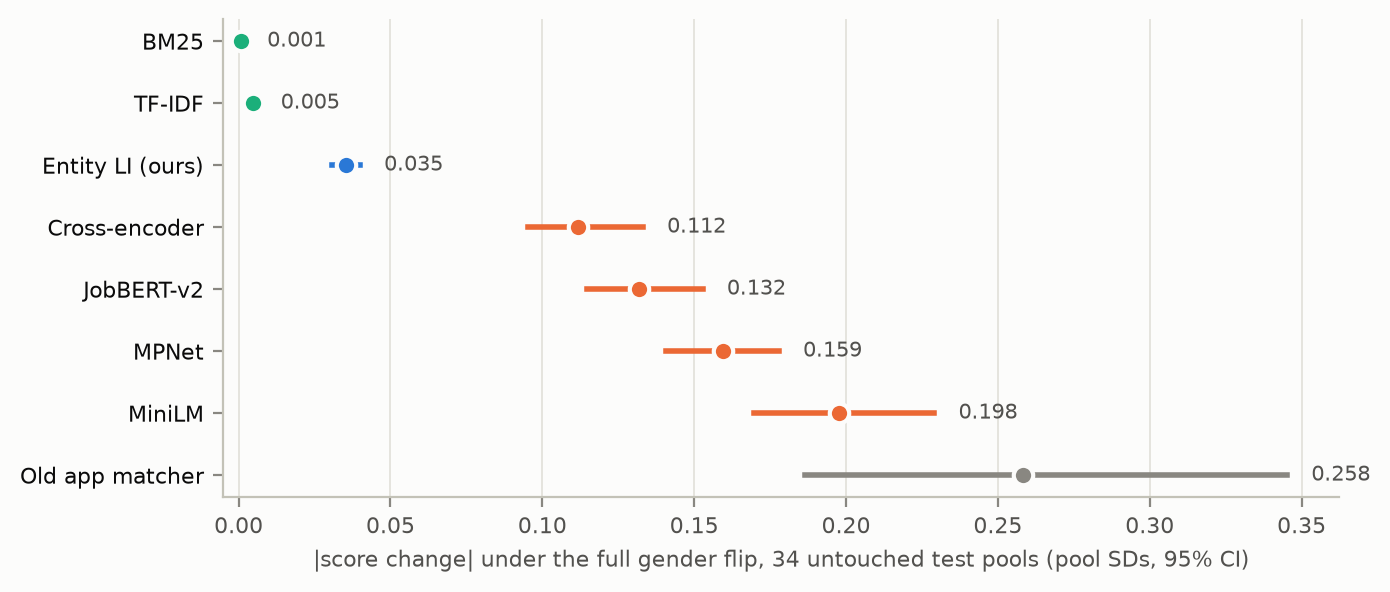
\includegraphics[width=\columnwidth]{figs/report_heldout.png}
\caption{The held-out check. The ordering of matchers is the same as on the full test set.}
\label{fig:7}
\end{figure}
\begin{table*}[!t]
\caption{Held-Out Check on 34 Untouched Test Pools}
\label{tab:21}
\centering
\footnotesize
\begin{tabularx}{\textwidth}{l>{\raggedright\arraybackslash}Xl>{\centering\arraybackslash}X}
\hline
\textbf{Matcher} & \textbf{nDCG@10, 34 fresh pools} & \textbf{Gap, 34 fresh pools} & \textbf{Gap, all 234 pools} \\
\hline
BM25 & 0.465 & 0.001 & 0.001 \\
TF-IDF & 0.458 & 0.005 & 0.005 \\
\textbf{Entity LI (ours)} & \textbf{0.544 [0.473, 0.611]} & \textbf{0.035 [0.031, 0.040]} & \textbf{0.033} \\
Cross-encoder & 0.325 & 0.112 & 0.121 \\
JobBERT-v2 & 0.653 & 0.132 & 0.126 \\
MPNet & 0.571 & 0.159 & 0.149 \\
MiniLM & 0.548 & 0.198 & 0.181 \\
Old app matcher & 0.446 & 0.258 & 0.272 \\
\hline
\end{tabularx}
\end{table*}
The fairness result replicates almost exactly (0.035 against 0.033). Accuracy is lower for every matcher on these 34 pools, so they are simply harder; our position relative to the others is unchanged, level with MiniLM and below JobBERT-v2. With 34 pools the accuracy intervals are wide.

\subsection{Near-Miss Suggestion Calibration}
\subsubsection{The question (RQ4)} The old app told users to ``consider reframing X to highlight Y'' whenever a job skill's best resume match had similarity between 0.35 and 0.55. Nobody had checked whether such suggestions were any good.

\subsubsection{A proxy for correctness} There are no gold labels for suggestions, so we used the ESCO hierarchy. Both sides are extracted with the ESCO ruler, so each phrase maps to a concept. A suggestion is:

\begin{itemize}
\item \textbf{strictly correct} if the two concepts are the same or one is the direct parent of the other;
\item \textbf{leniently correct} if strictly correct or the two share a direct parent (siblings).
\end{itemize}
Precision is the share of a band's suggestions that are correct. The proxy rewards taxonomic closeness only; it cannot say whether advice is useful to a candidate.

\subsubsection{The sweep} For relevant bio–job pairs, with MiniLM embeddings as in the old app, we computed precision for every band with lower bound 0.20–0.70 and upper bound 0.25–0.90 in steps of 0.05. The band was chosen on dev (highest lenient precision among bands with at least 100 dev suggestions) and evaluated on test.

\begin{figure}[!t]
\centering
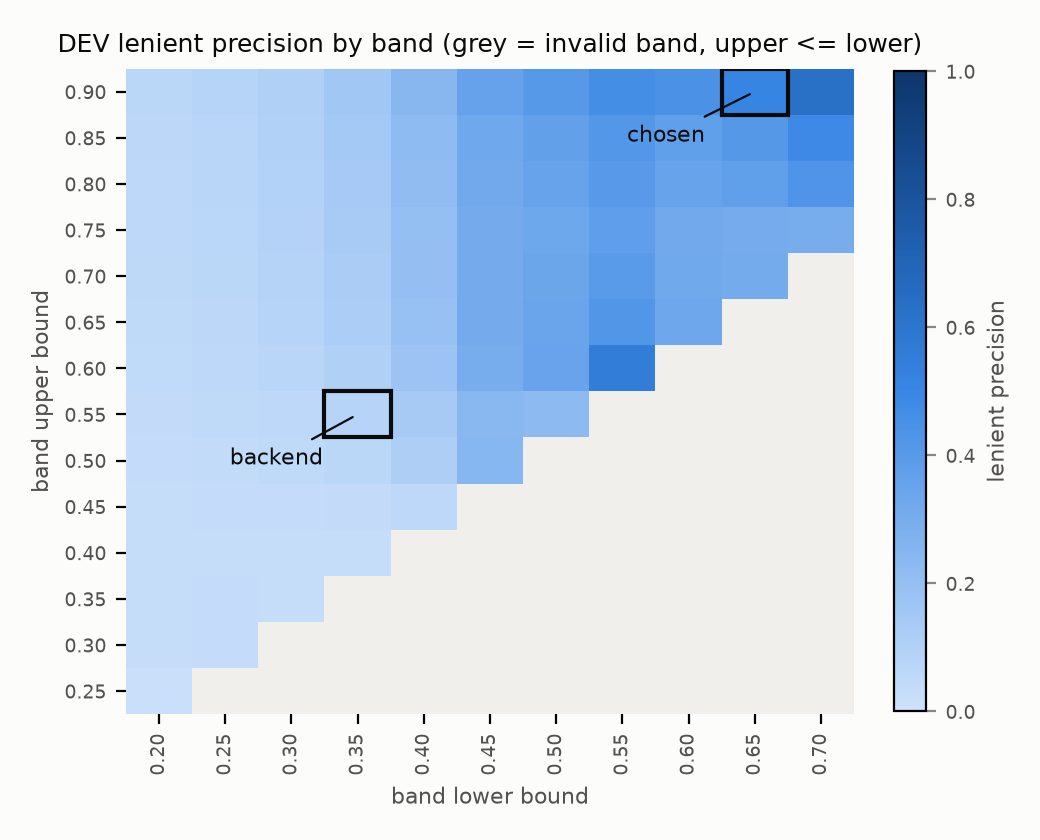
\includegraphics[width=\columnwidth]{figs/nearmiss_heatmap_dev.png}
\caption{Dev precision of every band. Precision rises with the lower bound; bands below 0.5 are near the base rate.}
\label{fig:8}
\end{figure}
\begin{figure*}[!t]
\centering
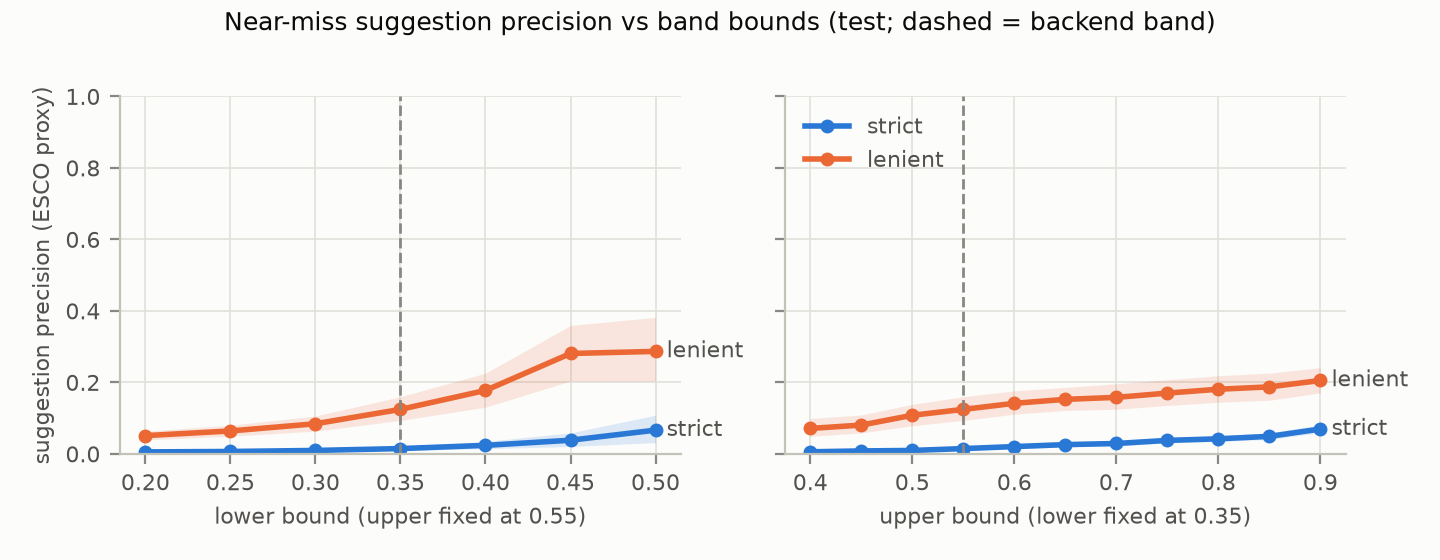
\includegraphics[width=0.9\textwidth]{figs/nearmiss_curves.png}
\caption{Test precision as one bound of the old band moves and the other stays fixed (dashed line = the old app's value). Raising either bound improves precision; shaded areas are 95\% intervals.}
\label{fig:9}
\end{figure*}
\begin{table}[!t]
\caption{Suggestion Precision by Band}
\label{tab:22}
\centering
\footnotesize
\begin{tabularx}{\columnwidth}{ll>{\centering\arraybackslash}Xc>{\centering\arraybackslash}X>{\centering\arraybackslash}X}
\hline
\textbf{Band} & \textbf{Split} & \textbf{Suggestions} & \textbf{Per pair} & \textbf{Strict precision} & \textbf{Lenient precision} \\
\hline
Old app, 0.35–0.55 & dev & 1,275 & 1.73 & 0.013 & 0.080 \\
Old app, 0.35–0.55 & test & 3,100 & 1.76 & 0.015 & 0.125 \\
Chosen, 0.65–0.90 & dev & 151 & 0.20 & 0.364 & 0.510 \\
Chosen, 0.65–0.90 & test & 362 & 0.21 & 0.483 & 0.707 \\
\hline
\end{tabularx}
\end{table}
\subsubsection{Findings} 

\begin{itemize}
\item \textbf{The old band is noise.} Its dev lenient precision (0.080) equals the base rate for all best matches (0.080). Its suggestions were no better than pairing a job skill with whichever resume phrase happened to be nearest.
\item \textbf{The chosen band sits above the old match threshold.} Pairs the old app counted as plain matches (above 0.55) are where the useful near-misses actually are.
\item \textbf{Precision and volume trade off.} The chosen band makes about one suggestion per five pairs instead of nearly two per pair, and on test 71\% are the same or a neighbouring ESCO concept.
\end{itemize}
The web application now uses the 0.65–0.90 band, computed exactly as in this sweep.

\subsection{Annotation Protocol and System Deployment}
\subsubsection{Why annotation} Relevance in this study means ``same occupation'', taken from BiasBios labels. That is a proxy for what a recruiter would judge. To test the proxy, and the matchers against human judgement, we built an annotation tool. Ratings have not yet been collected, so this section describes the instrument, not results.

\begin{itemize}
\item \textbf{Sample.} 250 bio–job pairs, stratified by consensus-score bin $\times$ job occupation $\times$ bio gender. The first draft sampled proportionally and came out 78\% obvious non-matches, which would waste annotator time and give no information about the hard cases. The final sample gives equal budget to three score bins cut at the 50\% and 90\% consensus quantiles. It contains 165, 35 and 50 pairs with graded label 0, 1 and 2.
\item \textbf{Scale.} 0 (no fit) to 3 (strong fit), with written guidelines and worked examples. Annotators are told to ignore names, pronouns and writing style.
\item \textbf{Tool.} A Streamlit app that shows only the two texts, in a per-annotator seeded order, and appends every rating to a CSV as it is made. Hidden strata and labels are kept in a separate file.
\item \textbf{Analysis, ready to run.} Cohen's kappa (including quadratic weights), ordinal Krippendorff's alpha, and the Spearman correlation of each matcher, and of the BiasBios label, with the mean human rating, all with bootstrap intervals.
\end{itemize}
\subsubsection{The web application} The last step was to make the application run what the paper tested.

\begin{itemize}
\item \textbf{Same code, not a copy.} The backend imports the research package and builds the final scorer from the same YAML. A test asserts that the application's score equals the research scorer's on the same input. Fitted statistics (the IDF table, dev calibration, the suggestion band) are exported from the final runs into one artifact file.
\item \textbf{Match endpoint.} Returns the score and, for every job requirement, its IDF weight, the closest resume skill, their similarity and the points lost. It also returns the entities read from the resume, so a user can see exactly what the matcher saw.
\item \textbf{Fairness check.} A new endpoint applies the paper's seven rewrites to the submitted resume and re-scores each version with our matcher, full-text MiniLM and the old app matcher, in the same pool-SD units as the paper.
\item \textbf{Research page.} Presents the data, training curves, headline chart, a per-perturbation explorer, significance tests, ablations, selection, the band heatmap, limitations and reproduction steps, all drawn from an export of the final runs.
\item \textbf{Privacy.} The research caches are switched off in the application, so submitted text is never written to disk.
\item \textbf{Bug fixes.} The three bias-checker bugs from the audit were fixed and covered by regression tests.
\end{itemize}
\subsubsection{What running it on real resumes taught us} Two things surfaced that the bios had hidden.

\begin{itemize}
\item Resumes have line breaks; bios do not. A header such as a name on one line and a title on the next was parsed as a single noun chunk. The application now ends each layout line as a sentence, which changes nothing on the research data.
\item On one test resume, swapping ``She'' for ``He'' moved our score more than MiniLM's ($-$0.156 against +0.023 pool SDs), because the contextual tagger changed which spans it extracted. This is the ablation finding of Section V-B appearing in a single case. One resume is an anecdote and the averaged result stands, but it shows the residual leak is real and where it comes from.
\end{itemize}
\subsection{Limitations and Threats to Validity}
\begin{table*}[!t]
\caption{Limitations and Mitigations}
\label{tab:23}
\centering
\footnotesize
\begin{tabularx}{\textwidth}{>{\raggedright\arraybackslash}X>{\raggedright\arraybackslash}X>{\raggedright\arraybackslash}X}
\hline
\textbf{Limitation} & \textbf{Why it matters} & \textbf{What we did about it} \\
\hline
Bios are not resumes & BiasBios texts are about 60 words, third person, and list credentials more than skills. Real resumes are longer and skill-dense. & Stated throughout; the app labels its score references as bio-based. Replication on real resumes is the most important next step. \\
Relevance is a proxy & ``Same occupation'' is not a recruiter's judgement of fit. & Annotation tool built; ratings pending. \\
Binary gender & The source labels are M/F only. & Nothing can be concluded about non-binary candidates. \\
Design informed by test data & The final method's candidate family came from ablations on 200 test pools. & Final choice on dev only by a pre-declared rule; 34 untouched pools replicate the result. Not a pre-registered design. \\
Ten occupations have no pools & Comedian, composer, DJ, filmmaker, model, painter, pastor, poet, rapper and yoga teacher had too few postings. & Reported; those bios still serve as irrelevant candidates. \\
Unreviewed title mappings & 1,114 ambiguous job titles were excluded pending human review. & Excluding them is conservative; the review file exists. \\
Underpowered conditions & Affiliation and agentic rewrites change 0.3\% and 2.5\% of bios. & Gaps reported over changed bios with intervals; conclusions about these conditions are weak. \\
Residual leakage & Noun chunks pass some names; ESCO treats agentic words as skills; the tagger reacts to context. & Measured in Sections V-A and V-B; shown to users in the app. \\
Unverified resources & The gender-coded word lists are not yet checked against Gaucher et al. \cite{gaucher}; Wikidata name labels contain some errors (for example a male name listed as female). & Flagged in code and in the app. \\
JobBERT-v2 out of design & It was trained on titles and skill lists, and is used on documents through 64-token windows. & Stated; it is still the most accurate baseline. \\
Missing baseline & The LLM judge was implemented but not run. & Listed as future work. \\
English, US postings, one seed for the tagger downstream & Results may not transfer to other languages, markets or tagger seeds. & Three tagger seeds agree on extraction quality; only seed 13 was used downstream. \\
One machine & All timings and runs are from a single consumer GPU. & Every run logs its environment and commit. \\
\hline
\end{tabularx}
\end{table*}
Two interpretive cautions apply. A small counterfactual gap means the score is insensitive to the cues we perturbed; it does not mean the matcher is fair in every sense. And lexical matchers' near-zero gaps come from discarding pronouns as stop-words, a blunt mechanism that also discards meaning.

\section{Conclusion}
We asked whether a resume matcher that only compares extracted skills leaks less demographic signal than one that reads the whole text. On 234 held-out job pools and seven counterfactual rewrites, the answer has two parts.

\subsubsection{Against full-text neural matchers, yes} Under a full gender flip the entity-level matcher's score moves by 0.033 pool standard deviations, against 0.121–0.181 for MiniLM, MPNet, JobBERT-v2 and a cross-encoder, and 0.272 for the application's original matcher. Candidates move about one rank in a hundred instead of four to ten. The differences are significant after correction, hold for pronouns, US names, Indian names and ethnicity-only name swaps, and replicate on 34 pools that no earlier experiment touched. Group metrics agree: the matcher shows no measurable gender gap in true-positive rate or top-10 exposure.

\subsubsection{Against lexical matchers, no} BM25 and TF-IDF are more invariant still, at lower accuracy.

\subsubsection{Accuracy is competitive, not best} At nDCG@10 0.619 the matcher is tied with MiniLM and MPNet and clearly above the lexical baselines and the original app, but 0.098 below full-text JobBERT-v2. A practitioner choosing between them is trading about ten points of nDCG for roughly a four-fold reduction in gender leakage.

\subsubsection{The mechanism is the extractor} A dictionary extractor is blind to pronouns but treats agentic words as skills. A learned tagger is more accurate but reacts to context, including pronouns. Adding filtered noun chunks improved accuracy, coverage and fairness together. Entity restriction is therefore not a guarantee; it moves the fairness question from the encoder to the extractor, where it is easier to inspect.

\subsubsection{A practical by-product} The original application's suggestion band was indistinguishable from chance. The replacement, chosen on development data, is correct by the ESCO proxy 71\% of the time on test.

\subsection{Future Work}
\begin{itemize}
\item Replicate on real resumes, where skill density is higher and the bio-specific coverage problem should shrink.
\item Collect the human ratings and report agreement and matcher–human correlation.
\item Reduce the tagger's context sensitivity, for example by training with counterfactual augmentation, and filter person names out of noun chunks.
\item Run the LLM-judge baseline and a second tagger seed downstream.
\item Extend perturbations beyond binary gender and two name pools.
\item Verify the gender-coded word lists against the source paper and complete the title-mapping review.
\end{itemize}
The code, configurations, tests, result summaries and figures are in the project repository, and the method runs in the accompanying web application, where anyone can repeat the audit on a resume of their own.


\balance
\begin{thebibliography}{99}
\item[] \emph{These entries were written from memory and have not been checked against the published versions. Verify authors, venues and years before submission.}
\bibitem{bertrand} M. Bertrand and S. Mullainathan, ``Are Emily and Greg more employable than Lakisha and Jamal? A field experiment on labor market discrimination,'' \emph{Amer. Econ. Rev.}, 2004.
\bibitem{wilson} K. Wilson and A. Caliskan, ``Gender, race, and intersectional bias in resume screening via language model retrieval,'' in \emph{Proc. AIES}, 2024.
\bibitem{colbert} O. Khattab and M. Zaharia, ``ColBERT: Efficient and effective passage search via contextualized late interaction over BERT,'' in \emph{Proc. SIGIR}, 2020.
\bibitem{bertscore} T. Zhang, V. Kishore, F. Wu, K. Weinberger, and Y. Artzi, ``BERTScore: Evaluating text generation with BERT,'' in \emph{Proc. ICLR}, 2020.
\bibitem{bm25} S. Robertson and H. Zaragoza, ``The probabilistic relevance framework: BM25 and beyond,'' \emph{Found. Trends Inf. Retr.}, 2009.
\bibitem{pjfnn} C. Zhu \emph{et al.}, ``Person-job fit: Adapting the right talent for the right job with joint representation learning,'' \emph{ACM Trans. Manage. Inf. Syst.}, 2018.
\bibitem{apjfnn} C. Qin \emph{et al.}, ``Enhancing person-job fit for talent recruitment: An ability-aware neural network approach,'' in \emph{Proc. SIGIR}, 2018.
\bibitem{sbert} N. Reimers and I. Gurevych, ``Sentence-BERT: Sentence embeddings using Siamese BERT-networks,'' in \emph{Proc. EMNLP}, 2019.
\bibitem{minilm} W. Wang \emph{et al.}, ``MiniLM: Deep self-attention distillation for task-agnostic compression of pre-trained transformers,'' in \emph{Proc. NeurIPS}, 2020.
\bibitem{mpnet} K. Song \emph{et al.}, ``MPNet: Masked and permuted pre-training for language understanding,'' in \emph{Proc. NeurIPS}, 2020.
\bibitem{monobert} R. Nogueira and K. Cho, ``Passage re-ranking with BERT,'' \emph{arXiv} preprint, 2019.
\bibitem{jobbert} J.-J. Decorte, J. Van Hautte, T. Demeester, and C. Develder, ``JobBERT: Understanding job titles through skills,'' in \emph{FEAST Workshop, ECML-PKDD}, 2021.
\bibitem{skillspan} M. Zhang, K. N. Jensen, S. D. Sonniks, and B. Plank, ``SkillSpan: Hard and soft skill extraction from English job postings,'' in \emph{Proc. NAACL}, 2022.
\bibitem{gaucher} D. Gaucher, J. Friesen, and A. C. Kay, ``Evidence that gendered wording in job advertisements exists and sustains gender inequality,'' \emph{J. Pers. Soc. Psychol.}, 2011.
\bibitem{madera} J. M. Madera, M. R. Hebl, and R. C. Martin, ``Gender and letters of recommendation for academia: Agentic and communal differences,'' \emph{J. Appl. Psychol.}, 2009.
\bibitem{dastin} J. Dastin, ``Amazon scraps secret AI recruiting tool that showed bias against women,'' \emph{Reuters}, 2018.
\bibitem{raghavan} M. Raghavan, S. Barocas, J. Kleinberg, and K. Levy, ``Mitigating bias in algorithmic hiring: Evaluating claims and practices,'' in \emph{Proc. FAT*}, 2020.
\bibitem{bolukbasi} T. Bolukbasi \emph{et al.}, ``Man is to computer programmer as woman is to homemaker? Debiasing word embeddings,'' in \emph{Proc. NeurIPS}, 2016.
\bibitem{biasbios} M. De-Arteaga \emph{et al.}, ``Bias in bios: A case study of semantic representation bias in a high-stakes setting,'' in \emph{Proc. FAT*}, 2019.
\bibitem{kusner} M. Kusner, J. Loftus, C. Russell, and R. Silva, ``Counterfactual fairness,'' in \emph{Proc. NeurIPS}, 2017.
\bibitem{lu} K. Lu, P. Mardziel, F. Wu, P. Amancharla, and A. Datta, ``Gender bias in neural natural language processing,'' \emph{arXiv} preprint, 2018.
\bibitem{zhao} J. Zhao, T. Wang, M. Yatskar, V. Ordonez, and K.-W. Chang, ``Gender bias in coreference resolution: Evaluation and debiasing methods,'' in \emph{Proc. NAACL}, 2018.
\bibitem{garg} S. Garg \emph{et al.}, ``Counterfactual fairness in text classification through robustness,'' in \emph{Proc. AIES}, 2019.
\bibitem{hardt} M. Hardt, E. Price, and N. Srebro, ``Equality of opportunity in supervised learning,'' in \emph{Proc. NeurIPS}, 2016.
\bibitem{singh} A. Singh and T. Joachims, ``Fairness of exposure in rankings,'' in \emph{Proc. KDD}, 2018.
\bibitem{mcsherry} F. McSherry and M. Najork, ``Computing information retrieval performance measures efficiently in the presence of tied scores,'' in \emph{Proc. ECIR}, 2008.
\bibitem{jobbertv2} TechWolf, ``JobBERT-v2,'' model card, Hugging Face (\texttt{TechWolf/\allowbreak{}JobBERT-\allowbreak{}v2}).
\bibitem{esco} European Commission, ``ESCO: European Skills, Competences, Qualifications and Occupations,'' v1.2.1.
\bibitem{ndcg} K. Järvelin and J. Kekäläinen, ``Cumulated gain-based evaluation of IR techniques,'' \emph{ACM Trans. Inf. Syst.}, 2002.
\bibitem{bootstrap} B. Efron and R. Tibshirani, \emph{An Introduction to the Bootstrap}. Chapman \& Hall, 1993.
\bibitem{holm} S. Holm, ``A simple sequentially rejective multiple test procedure,'' \emph{Scand. J. Statist.}, 1979.
\bibitem{cohen} J. Cohen, ``A coefficient of agreement for nominal scales,'' \emph{Educ. Psychol. Meas.}, 1960.
\bibitem{krippendorff} K. Krippendorff, \emph{Content Analysis: An Introduction to Its Methodology}. Sage, 2004.
\bibitem{d_biasbios} BiasBios dataset, \texttt{LabHC/\allowbreak{}bias\_\allowbreak{}in\_\allowbreak{}bios}, Hugging Face (MIT licence).
\bibitem{d_linkedin} LinkedIn Job Postings dataset, \texttt{arshkon/\allowbreak{}linkedin-\allowbreak{}job-\allowbreak{}postings}, Kaggle (CC BY-SA 4.0).
\bibitem{d_ssa} U.S. Social Security Administration, national baby-name counts (via the Hugging Face mirror \texttt{nkrishnaswami/\allowbreak{}us-\allowbreak{}ssa-\allowbreak{}baby-\allowbreak{}names-\allowbreak{}national}).
\bibitem{d_wikidata} Wikidata, given names of people with Indian citizenship (CC0); query archived in the project repository.
\end{thebibliography}

\end{document}
